%*******************************************************************************************%
%	   CONTRIBUIÇÕES À MODELAGEM DINAMICA E AO CONTROLE DE MANIPULADORES PARALELOS          %
% 																					   		%
% June 2015															 						%
% Author: Renato Maia Matarazzo Orsino														%
% bash modularmodelling.sh					 												%
% 																							%
%*******************************************************************************************%


\documentclass[25pt,landscape]{beamer}
	\mode<presentation> {
	  \usetheme{Warsaw}
	  \setbeamercovered{transparent}
	  \useoutertheme{shadow}
	  \useoutertheme{infolines}
	  \useinnertheme{rounded}
	  \setbeamertemplate{theorems}[numbered]
	  \setbeamertemplate{bibliography item}[text]
	  \usecolortheme{default}
	}


% - INPUT - %
\usepackage[T1]{fontenc}
\usepackage[latin1]{inputenc}
\usepackage[brazil]{babel}


% - MATH - %
\usepackage{amsmath,amsfonts,amssymb}
\usepackage{amsthm}
\usepackage{accents}


% - GENERAL - %
\usepackage{cmbright}
\usepackage{natbib}
\usepackage{color}
% \usepackage[pdftex,dvipsnames]{color}
% \usepackage{geometry}
\usepackage{array,hhline,supertabular,tabularx}
\usepackage{hyperref}
% \usepackage[colorlinks,citecolor=black,urlcolor=black,linkcolor=black]{hyperref}
\usepackage{graphicx}
% \usepackage[pdftex]{graphicx}
\usepackage{enumitem}
\usepackage{float}
\usepackage{titlesec}
\usepackage{pp4link}
\usepackage{mpmulti}
\usepackage{multimedia}
\usepackage[display]{texpower}
\usepackage[overlay,absolute]{textpos}
\setlength{\TPHorizModule}{1cm}
\setlength{\TPVertModule}{1cm}
\usepackage{multicol}
\usepackage{subfig}

% - SPECIAL - %
\usepackage{EXTRAS/special-char}
\usepackage{EXTRAS/special-conf}




%---------------------------------------------------------------------------------------%
%										BEAMER											%
%---------------------------------------------------------------------------------------%

\begin{document}


\begin{frame}
    \titlepage
\end{frame}

\begin{frame}{Introdução}
    \framesubtitle{Mecanismos paralelos}
    \pause
    \begin{block}{Caracter\'isticas Promissoras}
    	\pause
        \begin{itemize} 
            \item[--] Grande capacidade de carga \\[8pt]
            \item[--] Alta rigidez estrutural \\[8pt]
            \item[--] Alta precis\~ao de posicionamento \\[8pt]
            \item[--] Baixa in\'ercia \\[8pt]
            \item[--] Altas velocidades e acelera\c{c}\~oes \\[8pt]
        \end{itemize}
    \end{block}
    \pause
    \begin{block}{Inconvenientes}
    	\pause
        \begin{itemize}
        	\item[--] Grande n\'umero de componentes mec\^anicos \\[8pt]
            \item[--] Pequena \'area de trabalho \\[8pt]
            \item[--] Din\^amica complexa e n\~ao linear \\[8pt]
        \end{itemize}
    \end{block}
\end{frame}

\begin{frame}{Introdução}
    \framesubtitle{Mecanismos paralelos}
    \begin{block}{Aplica\c{c}\~oes}
        \begin{itemize}
            \item[--] Pick-and-place
        \end{itemize}
    \end{block}
    \begin{figure}[!h]
        \centering
        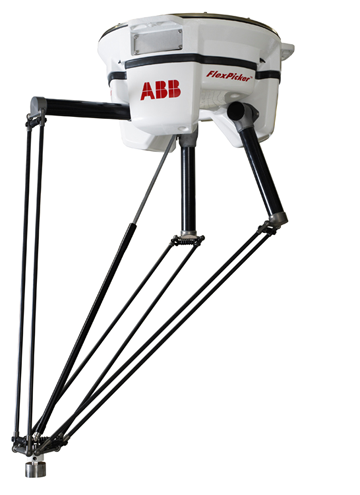
\includegraphics[scale=0.35]{ABB-Flexpicker-Robot.png}
    \end{figure}  
\end{frame}

\begin{frame}{Introdução}
    \framesubtitle{Mecanismos paralelos}
    \begin{block}{Aplica\c{c}\~oes}
        \begin{itemize}
            \item[--] Simuladores
        \end{itemize}
    \end{block}
    \begin{figure}[!h]
        \centering
        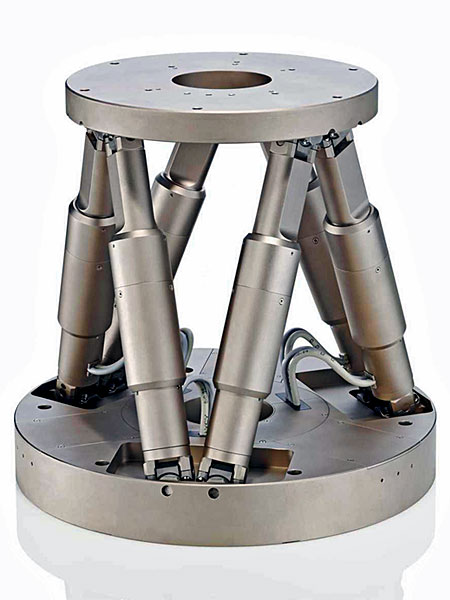
\includegraphics[scale=0.30]{hexapods.jpg}
    \end{figure}  
\end{frame}

\begin{frame}{Introdução}
    \framesubtitle{Mecanismos paralelos}
    \begin{block}{Aplica\c{c}\~oes}
        \begin{itemize}
            \item[--] Usinagem
        \end{itemize}
    \end{block}
    \begin{figure}[!h]
        \centering
        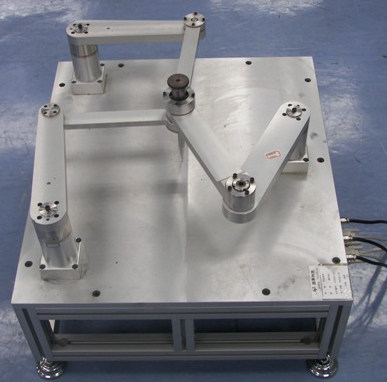
\includegraphics[scale=0.60]{image44.png}
    \end{figure}  
\end{frame}

%Grupo de pesquisa

\begin{frame}{Introdução}
	\framesubtitle{Grupo de pesquisa}
	\pause
	\begin{block}{LaMMaR}
		Laborat\'orio de Mecanismos, M\'aquinas e Rob\^os
    \end{block}
    \begin{figure}[!h]
        \centering
        \includegraphics[scale=0.25]{LaMMaR.png}
    \end{figure}
\end{frame}

\begin{frame}{Introdução}
	\framesubtitle{Grupo de pesquisa}
	\begin{block}{Rob\^os}
		Giovanna
    \end{block}
    \begin{figure}[!h]
        \centering
        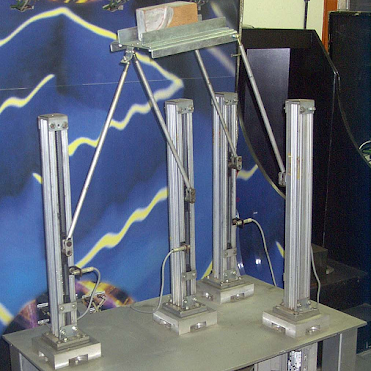
\includegraphics[scale=0.33]{Giovanna.png}
    \end{figure}
\end{frame}

\begin{frame}{Introdução}
	\framesubtitle{Grupo de pesquisa}
	\begin{block}{Rob\^os}
		Dora
    \end{block}
    \begin{figure}[!h]
        \centering
        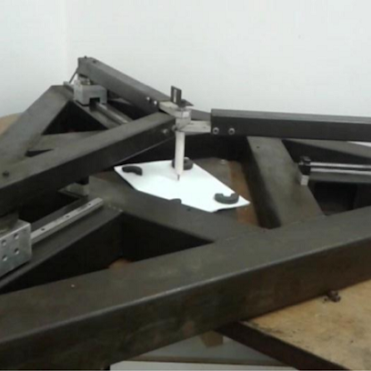
\includegraphics[scale=0.33]{Dora.png}
    \end{figure}
\end{frame}

\begin{frame}{Introdução}
	\framesubtitle{Grupo de pesquisa}
	\begin{block}{Rob\^os}
		Laila
    \end{block}
    \begin{figure}[!h]
        \centering
        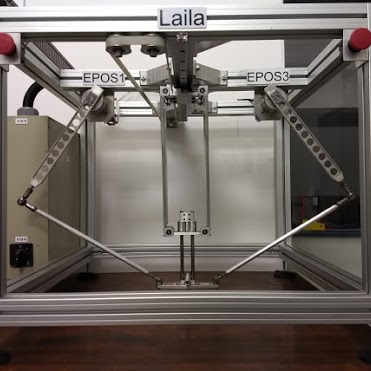
\includegraphics[scale=0.33]{Laila.jpg}
    \end{figure}
\end{frame}

\begin{frame}{Introdução}
	\framesubtitle{Grupo de pesquisa}
	\begin{block}{Rob\^os}
		Clara
    \end{block}
    \begin{figure}[!h]
        \centering
        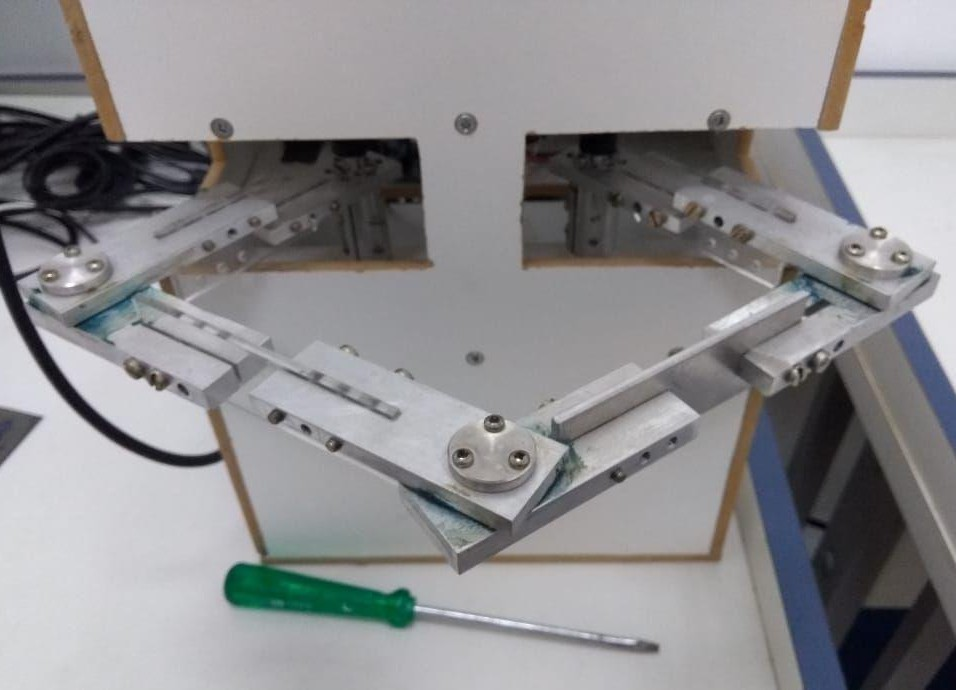
\includegraphics[scale=0.21]{Clara2.jpg}
    \end{figure}
\end{frame}

\begin{frame}{Objetivos}
	\pause
	\begin{block}{Geral}
		Contribuir para o aumento do desempenho de manipuladores paralelos
	\end{block}
	\pause
	\begin{exampleblock}{Como?}
		\pause
		\begin{itemize}
			\item[$\bullet$] Automatização do processo de modelagem dinâmica \\[8pt]
			\pause
			\item[$\bullet$] Emprego de técnicas de controle robusto baseado em modelo \\[8pt]
			\pause
			\item[$\bullet$] Compara\c{c}\~ao de desempenho das leis de controle propostas com as leis de controle mais encontradas na literatura, atrav\'es de ensaios experimentais \\[8pt]
		\end{itemize}
	\end{exampleblock}
\end{frame}

%============================================== REVISÃO DA LITERATURA =======================================================%


\begin{frame}{Revisão da Literatura}
    \framesubtitle{Modelagem Dinâmica}
    \pause
        \begin{block}{Influência da topologia do robô}
    	\begin{itemize}
    		\pause
    		\item[$\bullet$] Seriais
    		\begin{itemize}
    			\pause
    			\item[--] Cadeia aberta \\[4pt]
    			\item[--] Juntas ativas de 1 gl \\[4pt]
    			\item[--] N$^\circ$ de coord. gen. = N$^\circ$ atuadores = mobilidade \\[4pt]
    			\item[--] Conjunto mínimo de coord. generalizadas \\[4pt]
    			\item[--] Cinemática direta simples \\[4pt]
    			\item[--] Cinemática inversa complexa \\[4pt]
    			\item[--] Dinâmica direta - Sistema de EDOs \\[4pt]
    			\item[--] Dinâmica inversa - Sistema linear \\[4pt]
    			\item[--] Algoritmos recursivos para mod. dinâmica \\[4pt]
    		\end{itemize}
    	\end{itemize}
    \end{block}
    $$ $$
\end{frame}

\begin{frame}{Revisão da Literatura}
    \framesubtitle{Modelagem Dinâmica}
    \begin{block}{Influência da topologia do robô}
    	\begin{itemize}
    		\item[$\bullet$] Paralelos
    		\begin{itemize}
    			\pause
    			\item[--] Cadeia fechada \\[4pt]
    			\item[--] Juntas de 1, 2 ou 3 gl, ativas ou passivas \\[4pt]
    			\item[--] Grande número de elos \\[4pt]
    			\item[--] Grande quantidade de variáveis cinemáticas \\[4pt]
    			\item[--] Variáveis independentes e dependentes \\[4pt]
    			\item[--] Cinemática direta complexa \\[4pt]
    			\item[--] Cinemática inversa "simples" \\[4pt]
    			\item[--] Dinâmica direta - Sistema de EDAs ou EDOs \\[4pt]
    			\item[--] Dinâmica inversa - Sistema não linear \\[4pt]
    			\item[--] Coord. gen. ind.: coord. dos atuadores ou do efetuador \\[4pt]
    		\end{itemize}
    	\end{itemize}
    \end{block}
\end{frame}

\begin{frame}{Revisão da Literatura}
    \framesubtitle{Modelagem Dinâmica}
    \begin{block}{Dinâmica direta - EDAs}
		\begin{equation} \label{DAE1} \tag{2.1}
			\mM \, \ddot{\mq} + \mA^\msT \,\mlambda = \meta
		\end{equation}
		\begin{equation} \label{DAE2} \tag{2.2}
			\bar{\mq} \, (\mq,t) \, = \, \mzr
		\end{equation}
	
		Sendo
		\begin{equation} \tag{2.3}
			\mA(\mq,t) = \frac{\partial \bar{\mq}}{\partial \mq}
		\end{equation}
	\end{block}
\end{frame}

\begin{frame}{Revisão da Literatura}
    \framesubtitle{Modelagem Dinâmica}	
	\begin{block}{Dinâmica direta - EDOs}	
		\begin{equation} \label{DAE3} \tag{2.4}
			\underbrace{\left[ \begin{array}{cc}
			\mM & \mA^\msT \\
			\mA & \mzr
			\end{array}
			\right]}_{\mY}
			\left[ \begin{array}{c}
			\ddot{\mq} \\
			\mlambda
			\end{array}
			\right] =
			\left[ \begin{array}{c}
			\meta \\
			-\mb
			\end{array}
			\right]
		\end{equation}
		Sendo
	\begin{equation} \tag{2.5}
		\mb = \frac{\partial (\mA \dot{\mq})}{\partial \mq} \, \dot{\mq} + 2 \frac{\partial \mA}{\partial t} \, \dot{\mq} + \frac{\partial^2 \bar{\mq}}{\partial t^2}
	\end{equation}
	\end{block}
	\pause
	\begin{block}{Método estabilização de Baumgarte}
		\begin{equation} \label{baumgarte} \tag{2.6}
			\mb' = \mb + 2\hat{\alpha} \dot{\bar{\mq}} + \hat{\beta}^2 \bar{\mq}
		\end{equation}
	\end{block}	
\end{frame}

\begin{frame}{Revisão da Literatura}
    \framesubtitle{Modelagem Dinâmica}
        \begin{block}{Propósito}
    	\begin{itemize}
    		\pause
    		\item[$\bullet$] Simulação
    		\begin{itemize}
    			\pause
    			\item[--] Projeto/Dimensionamento do mecanismo/manipulador \\[4pt]
    			\item[--] Grau de detalhamento do modelo depende da aplicação \\[4pt]
    			\item[--] Não necessita rodar em tempo real \\[4pt]
    		\end{itemize}
    		\pause
    		\item[$\bullet$] Controle
    		\begin{itemize}
    			\pause
    			\item[--] Projeto do controlador \\[4pt]
    			\item[--] Compensação de não linearidades \\[4pt]
    			\item[--] Modelos demasiadamente complexos dificultam o projeto e podem aumentar o custo computacional \\[4pt]
    			\item[--] Modelos muito simplistas podem comprometer o desempenho \\[4pt]
    			\item[--] Muitas vezes precisa rodar em tempo real \\[4pt]
    		\end{itemize}
    	\end{itemize}
    \end{block}
\end{frame}

\begin{frame}{Revisão da Literatura}
    \framesubtitle{Modelagem Dinâmica}
    \begin{block}{Principais formulações}
        \begin{itemize}
            \item[$\bullet$] Formalismo de Newton-Euler (Arian \emph{et al.}, 2017; Zhang \emph{et al.}, 2014) \\[4pt] % Dasgupta e Mruthyunjaya, 1998; Li \emph{et al.}, 2003; Shiau \emph{et al.}, 2008;
            \item[$\bullet$] Formalismo de Lagrange (Singh e Santhakumar, 2015; Yao \emph{et al.}, 2017) \\[4pt] %Li e Xu, 2005; Singh \emph{et al.}, 2015; Singh \emph{et al.}, 2014;
            \item[$\bullet$] Princípio dos Trabalhos/Potências Virtuais (Gallardo-Alvarado \emph{et al.}, 2018; Li e Staicu, 2012) \\[4pt] %Codourey, 1996; Codourey e Burdet, 1997; Geike e McPhee, 2003; Li e Xu, 2009; Staicu, 2009; Staicu e Carp-Ciocardia, 2003; Staicu \emph{et al.}, 2007; Staicu e Zhang, 2008; Staicu \emph{et al.}, 2006; Wu \emph{et al.}, 2009; Zhao e Gao, 2009; Zhu \emph{et al.}, 2005;
            \item[$\bullet$] Formulação Lagrange-D'Alambert (Cheng \emph{et al.}, 2001; Yen e Lai, 2009) \\[4pt]
            \item[$\bullet$] Método de Kane (Ben-Horina \emph{et al.}, 1998; Shukla e Karki, 2014) \\[4pt]
            \item[$\bullet$] Formalismo de Boltzmann-Hammel (Abdellatif e Heimann, 2009; Altuzarra \emph{et al.}, 2015) \\[4pt]
            \item[$\bullet$] Formulação do Complemento Ortogonal Natural  (Akbarzadeh \emph{et al.}, 2013; Khan \emph{et al.}, 2005) \\[4pt] %Xi e Sinatra, 2002; 
        \end{itemize}
    \end{block}
\end{frame}

\begin{frame}{Revisão da Literatura}
    \framesubtitle{Controle}
    	\pause
        \begin{block}{Propósito}
    	\begin{itemize}
    		\pause
    		\item[$\bullet$] Controle ponto a ponto
    		\begin{itemize}
    			\pause
    			\item[--] \emph{Pick-and-place} \\[6pt]
    		\end{itemize}
    		\pause
    		\item[$\bullet$] Controle de trajetória
    		\begin{itemize}
    			\pause
    			\item[--] Usinagem \\[6pt]
    			\item[--] Soldagem \\[6pt]
    			\item[--] Aplicação de adesivos/selantes \\[6pt]
    			\item[--] Simuladores de voo/automobilísticos \\[6pt]
    		\end{itemize}
    	\end{itemize}
    \end{block}
\end{frame}

\begin{frame}{Revisão da Literatura}
    \framesubtitle{Controle}
    \pause
    \begin{block}{Principais técnicas}
        \begin{itemize}
            \item[$\bullet$] Controle Proporcional-Integral-Derivativo \\
            \item[$\bullet$] Controle por Torque Computado (Shang e Cong, 2009; Yen e Lai, 2009) \\ % Cheng \emph{et al.}, 2003; Li e Wu, 2004; Li e Xu, 2009;  (22; 55; 56; 75; 106)
            \item[$\bullet$] Controle por Torque Computado com pré-alimentação (Siciliano \emph{et al.}, 2010; Spong \emph{et al.}, 2006)\\  % Khalil e Dombre, 2002;  (48; 78; 85)
            \item[$\bullet$] Controle por Torque Computado Estendido (Zubizarreta \emph{et al.}, 2013; Zubizarreta \emph{et al.}, 2012) \\ % Zubizarreta \emph{et al.}, 2010; Zubizarreta \emph{et al.}, 2008;(113; 114; 115; 116)
            \item[$\bullet$] Controle Preditivo Baseado em Modelo (Duchaine \emph{et al.}, 2007; Vivas e Poignet, 2005) \\ %(32, 100)
            \item[$\bullet$] Controle Adaptativo (Chemori \emph{et al.}, 2013; Honegger \emph{et al.}, 2000)  \\ %Codourey e Burdet, 1997; Slotine e Li, 1987; (19; 25; 41; 84)
            \item[$\bullet$] Controle por Modos Deslizantes (Hu e Woo, 2006; Sadati e Ghadami, 2008)  \\ % Begon \emph{et al.}, 1995; Ertugrul e Kaynak, 2000; (9; 34; 42; 73)
        \end{itemize}
    \end{block}
\end{frame}

\begin{frame}{Revisão da Literatura}
    \framesubtitle{Controle}
    \begin{block}{Controle Proporcional-Integral-Derivativo (PID)}
        \begin{itemize}
            \item[$\bullet$] Técnica de controle linear descentralizado \\[8pt]
            \item[$\bullet$] Não baseado no modelo dinâmico do mecanismo \\[8pt]
            \item[$\bullet$] Simples implementação \\[8pt]
            \item[$\bullet$] Baixo custo computacional \\[8pt]
            \item[$\bullet$] Desempenho bastante limitado \\[8pt]
        \end{itemize}
    \end{block}
\end{frame}

\begin{frame}{Revisão da Literatura}
    \framesubtitle{Controle}
    \begin{figure}[!h]
        \centering
        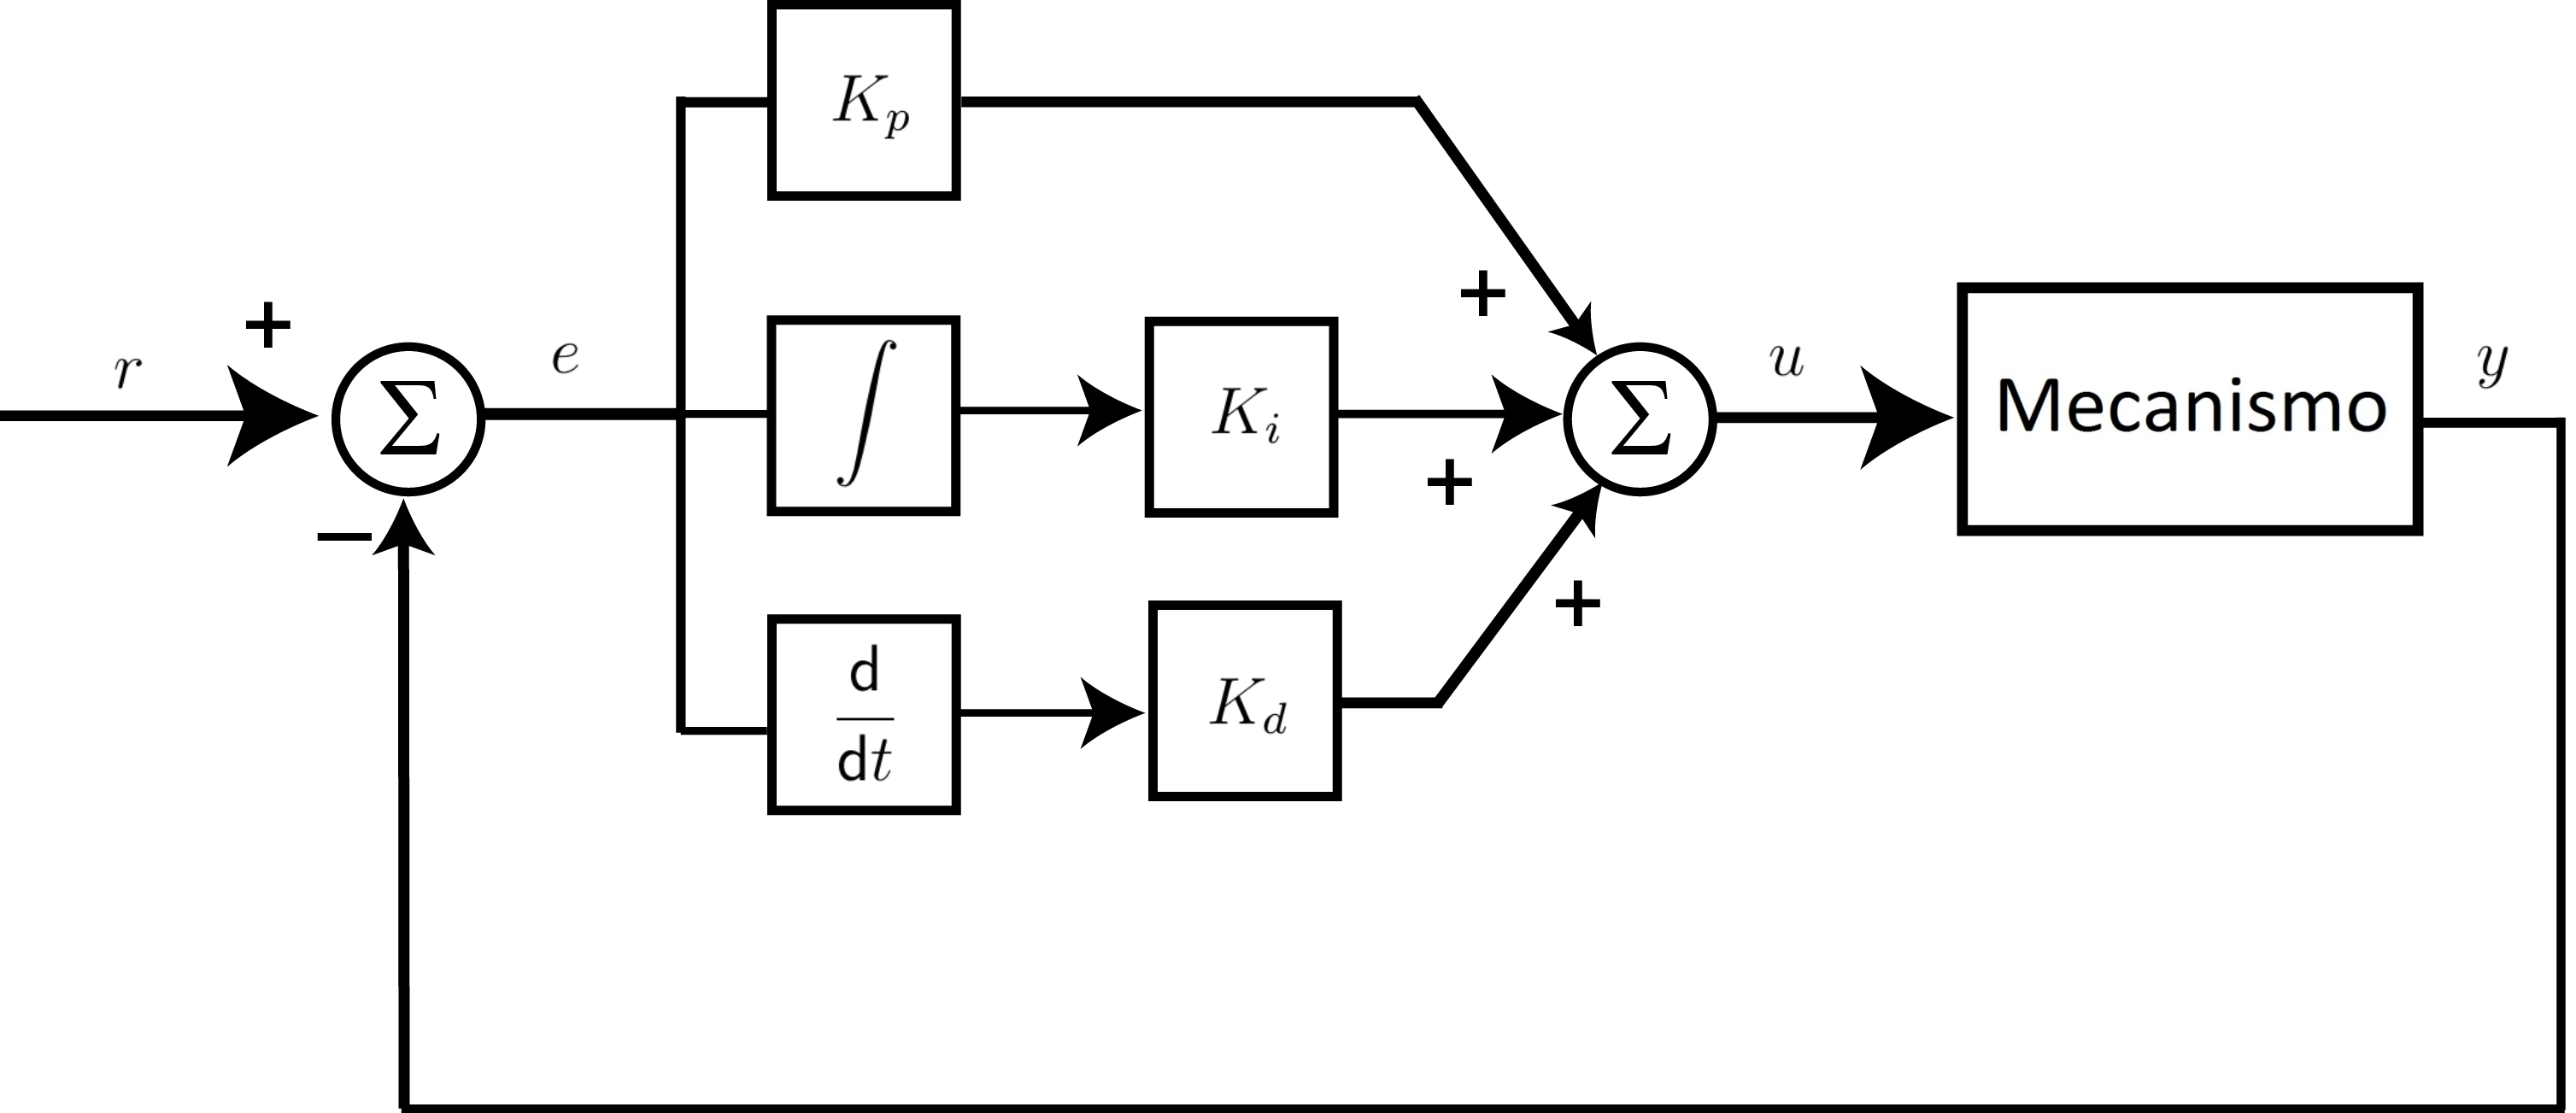
\includegraphics[scale=0.38]{PID.jpg}
    \end{figure}  
\end{frame}

\begin{frame}{Revisão da Literatura}
    \framesubtitle{Controle}
    \begin{block}{Controle por Torque Computado (CTC)}
        \begin{itemize}
            \item[$\bullet$] Técnica de controle não linear multivariável \\[8pt]
            \item[$\bullet$] Baseado no modelo dinâmico do mecanismo \\[8pt]
            \item[$\bullet$] Possui uma malha interna de compensação de não linearidades por realimentação e uma malha externa de PID \\[8pt]
            \item[$\bullet$] Desempenho superior ao PID simples, porém bastante dependente da qualidade do modelo dinâmico \\[8pt]
            \item[$\bullet$] Implementação mais complexa \\[8pt]
            \item[$\bullet$] Maior custo computacional \\[8pt]
        \end{itemize}
    \end{block}
\end{frame}

\begin{frame}{Revisão da Literatura}
    \framesubtitle{Controle}
    \begin{figure}[!h]
        \centering
        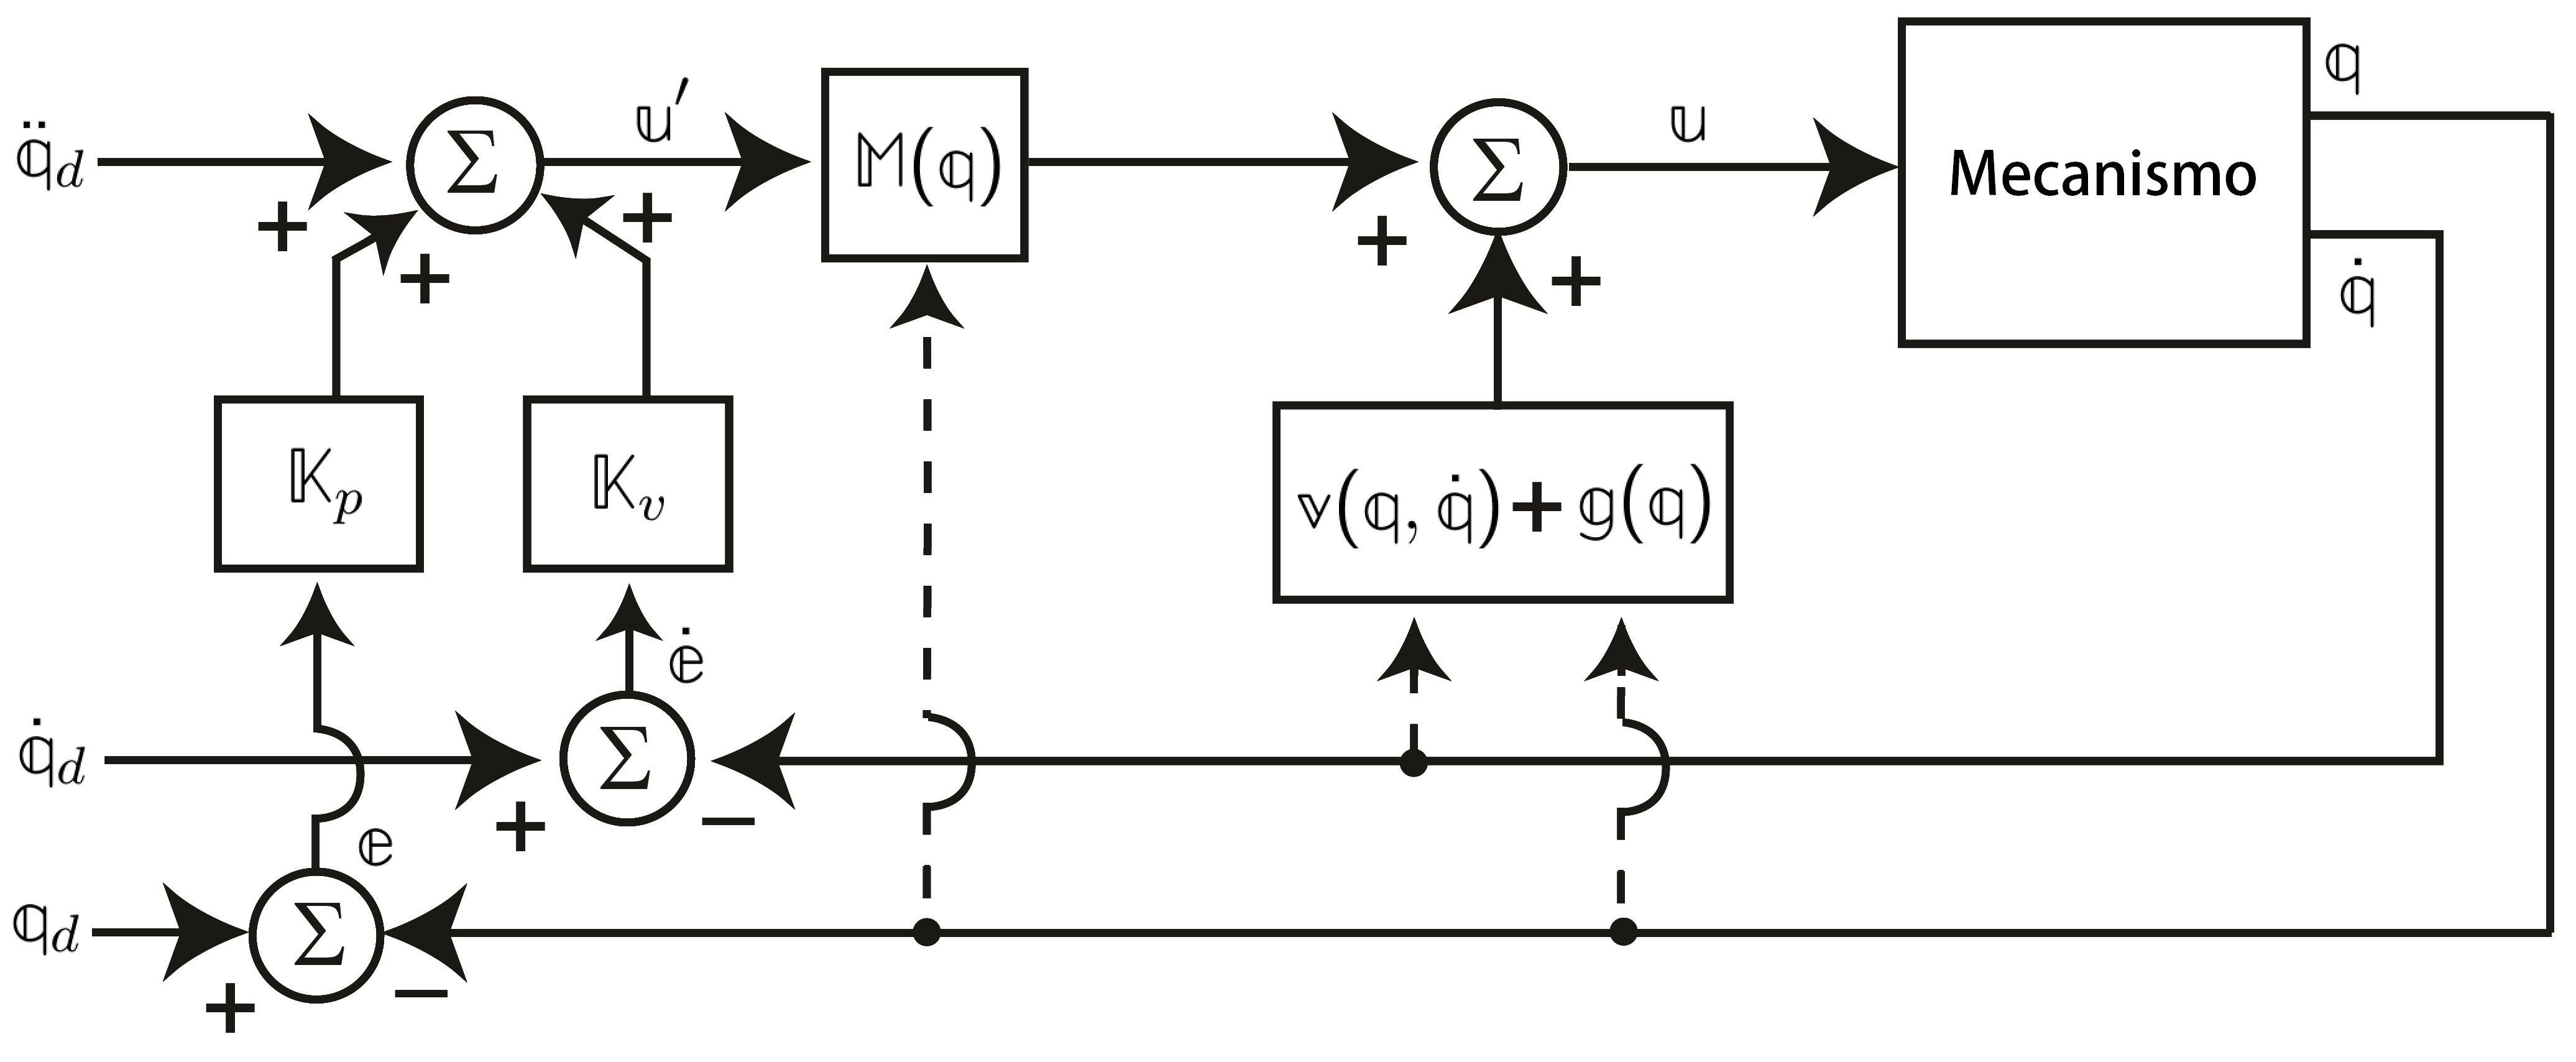
\includegraphics[scale=0.30]{CTC.jpg}
    \end{figure}  
\end{frame}

\begin{frame}{Revisão da Literatura}
    \framesubtitle{Controle}
    \begin{block}{Controle por Torque Computado com pré-alimentação (CTCp)}
        \begin{itemize}
            \item[$\bullet$] Lei de controle similar ao CTC \\[8pt]
            \item[$\bullet$] Realiza compensação de não linearidades por pré-alimentação \\[8pt]
            \item[$\bullet$] Menor custo computacional em relação ao CTC \\[8pt]
            \item[$\bullet$] Implementação mais simples que o CTC \\[8pt]
            \item[$\bullet$] Menor robustez em relação ao CTC \\[8pt]
        \end{itemize}
    \end{block}
\end{frame}

\begin{frame}{Revisão da Literatura}
    \framesubtitle{Controle}
    \begin{figure}[!h]
        \centering
        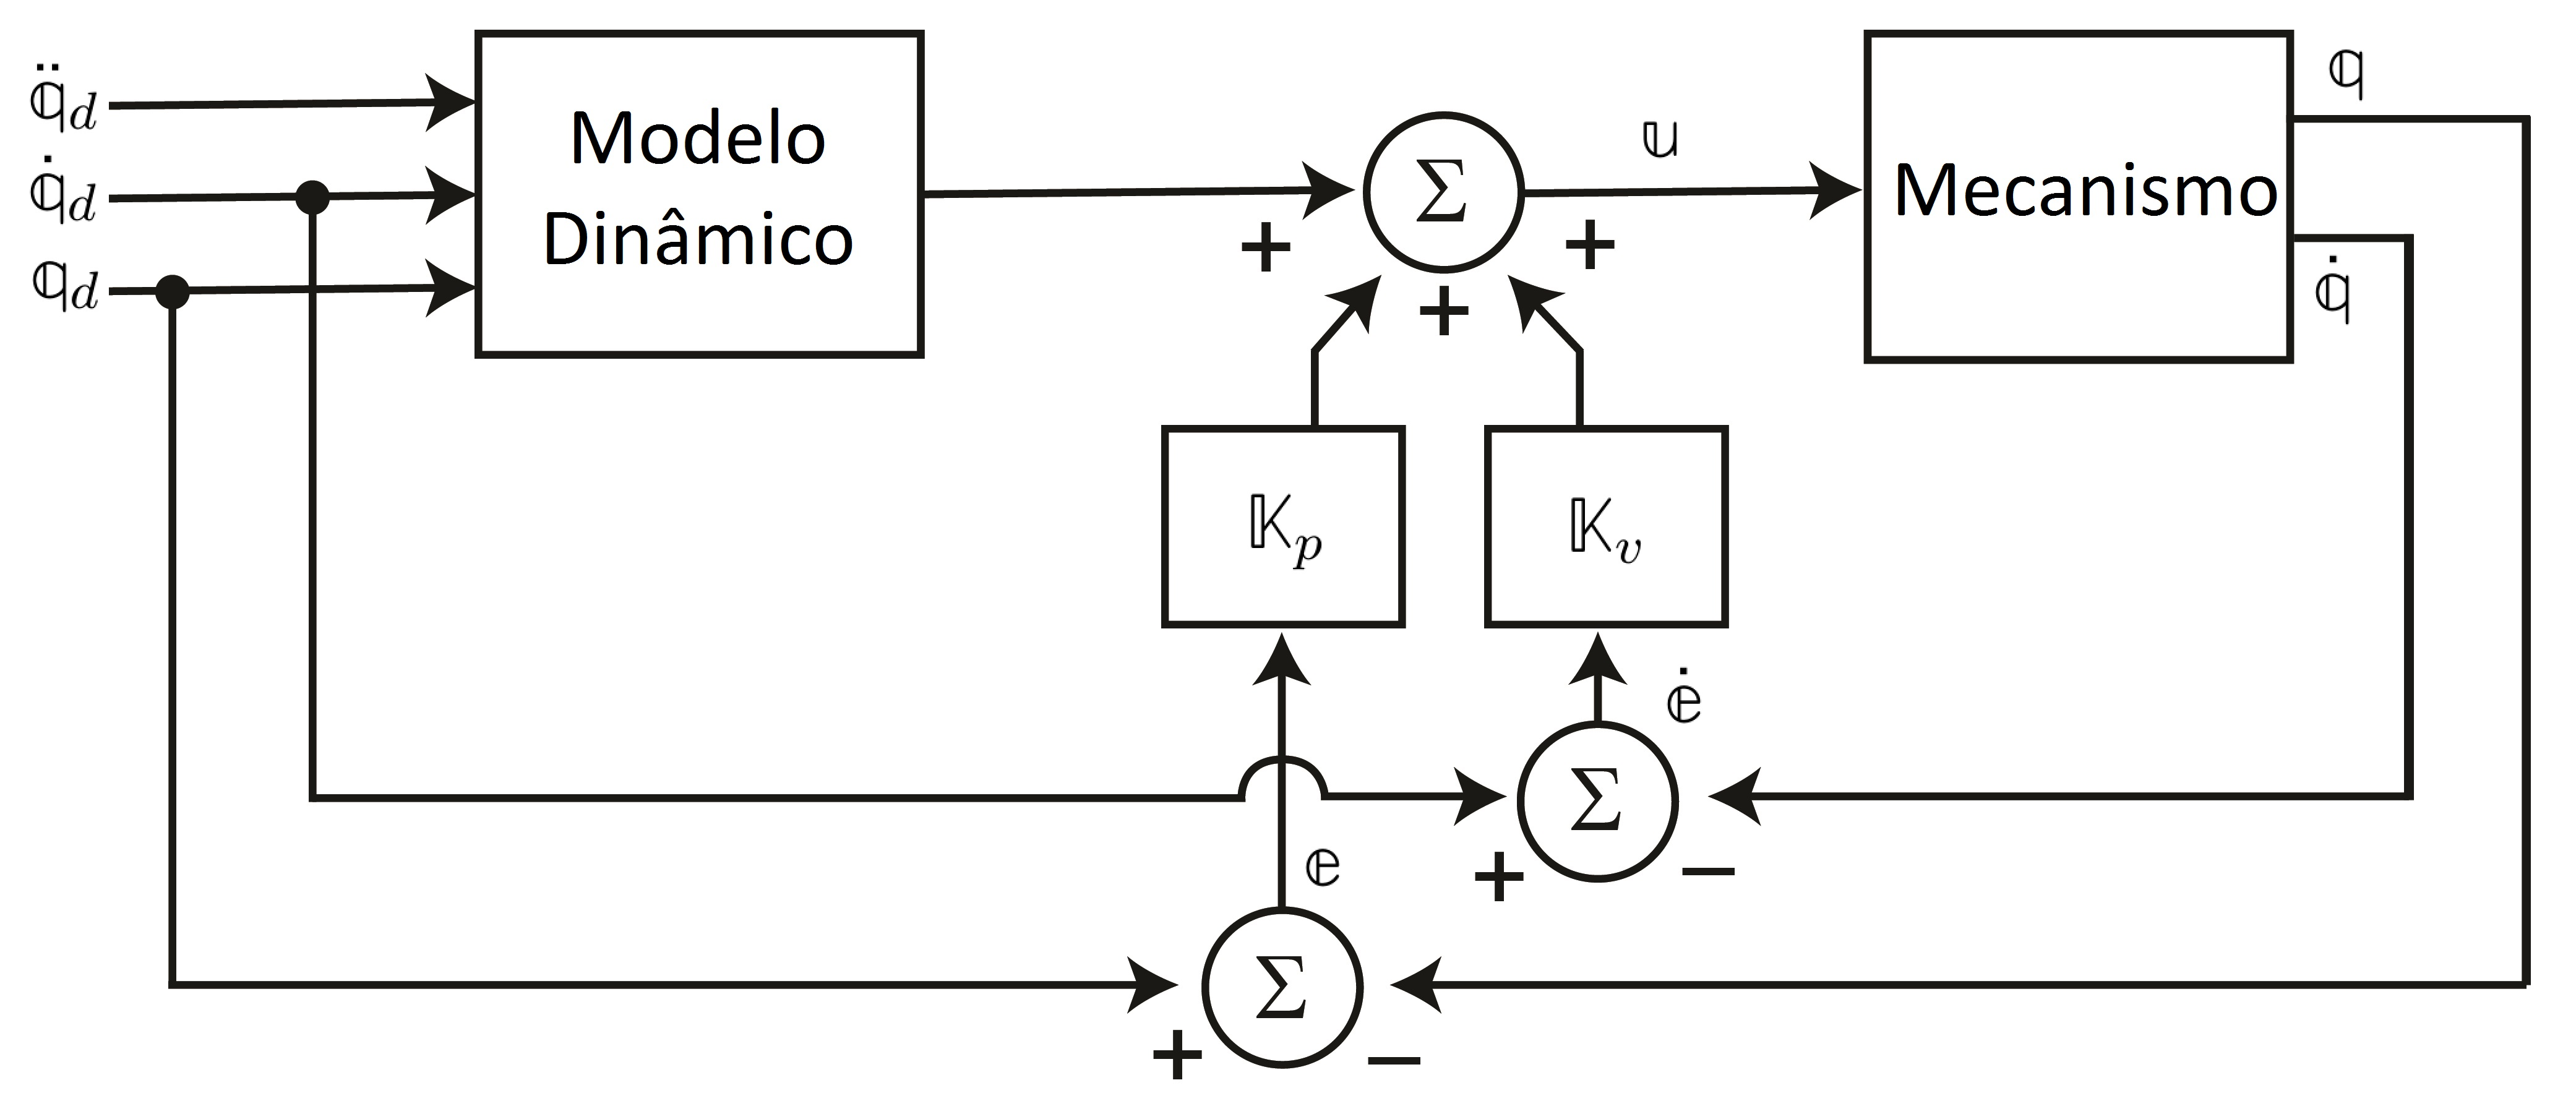
\includegraphics[scale=0.30]{CTCp.jpg}
    \end{figure}  
\end{frame}

\begin{frame}{Revisão da Literatura}
    \framesubtitle{Controle}
    \begin{block}{Controle por Torque Computado Estendido (CTCe)}
        \begin{itemize}
            \item[$\bullet$] Lei de controle similar ao CTC \\[8pt]
            \item[$\bullet$] Realiza compensação de não linearidades por realimentação \\[8pt]
            \item[$\bullet$] Utiliza informação redundante obtida pelo sensoriamento de juntas passivas na lei de controle \\[8pt]
            \item[$\bullet$] Maior robustez a incertezas paramétricas \\[8pt]
        \end{itemize}
    \end{block}
\end{frame}

\begin{frame}{Revisão da Literatura}
    \framesubtitle{Controle}
    \begin{block}{Controle Preditivo Baseado em Modelo (CPM)}
        \begin{itemize}
            \item[$\bullet$] Técnica de controle multi-variável baseado em modelo \\[8pt]
            \item[$\bullet$] Muito utilizado no controle de processos industriais \\[8pt]
            \item[$\bullet$] Realiza otimização em tempo real de uma função custo que envolve o erro e o esforço de controle em tempo futuro \\[8pt]
            \item[$\bullet$] Custo computacional bastante dependente da complexidade do modelo \\[8pt]
            \item[$\bullet$] Boa robustez a incertezas paramétricas  \\[8pt]
        \end{itemize}
    \end{block}
\end{frame}

\begin{frame}{Revisão da Literatura}
    \framesubtitle{Controle}
    \begin{figure}[!h]
        \centering
        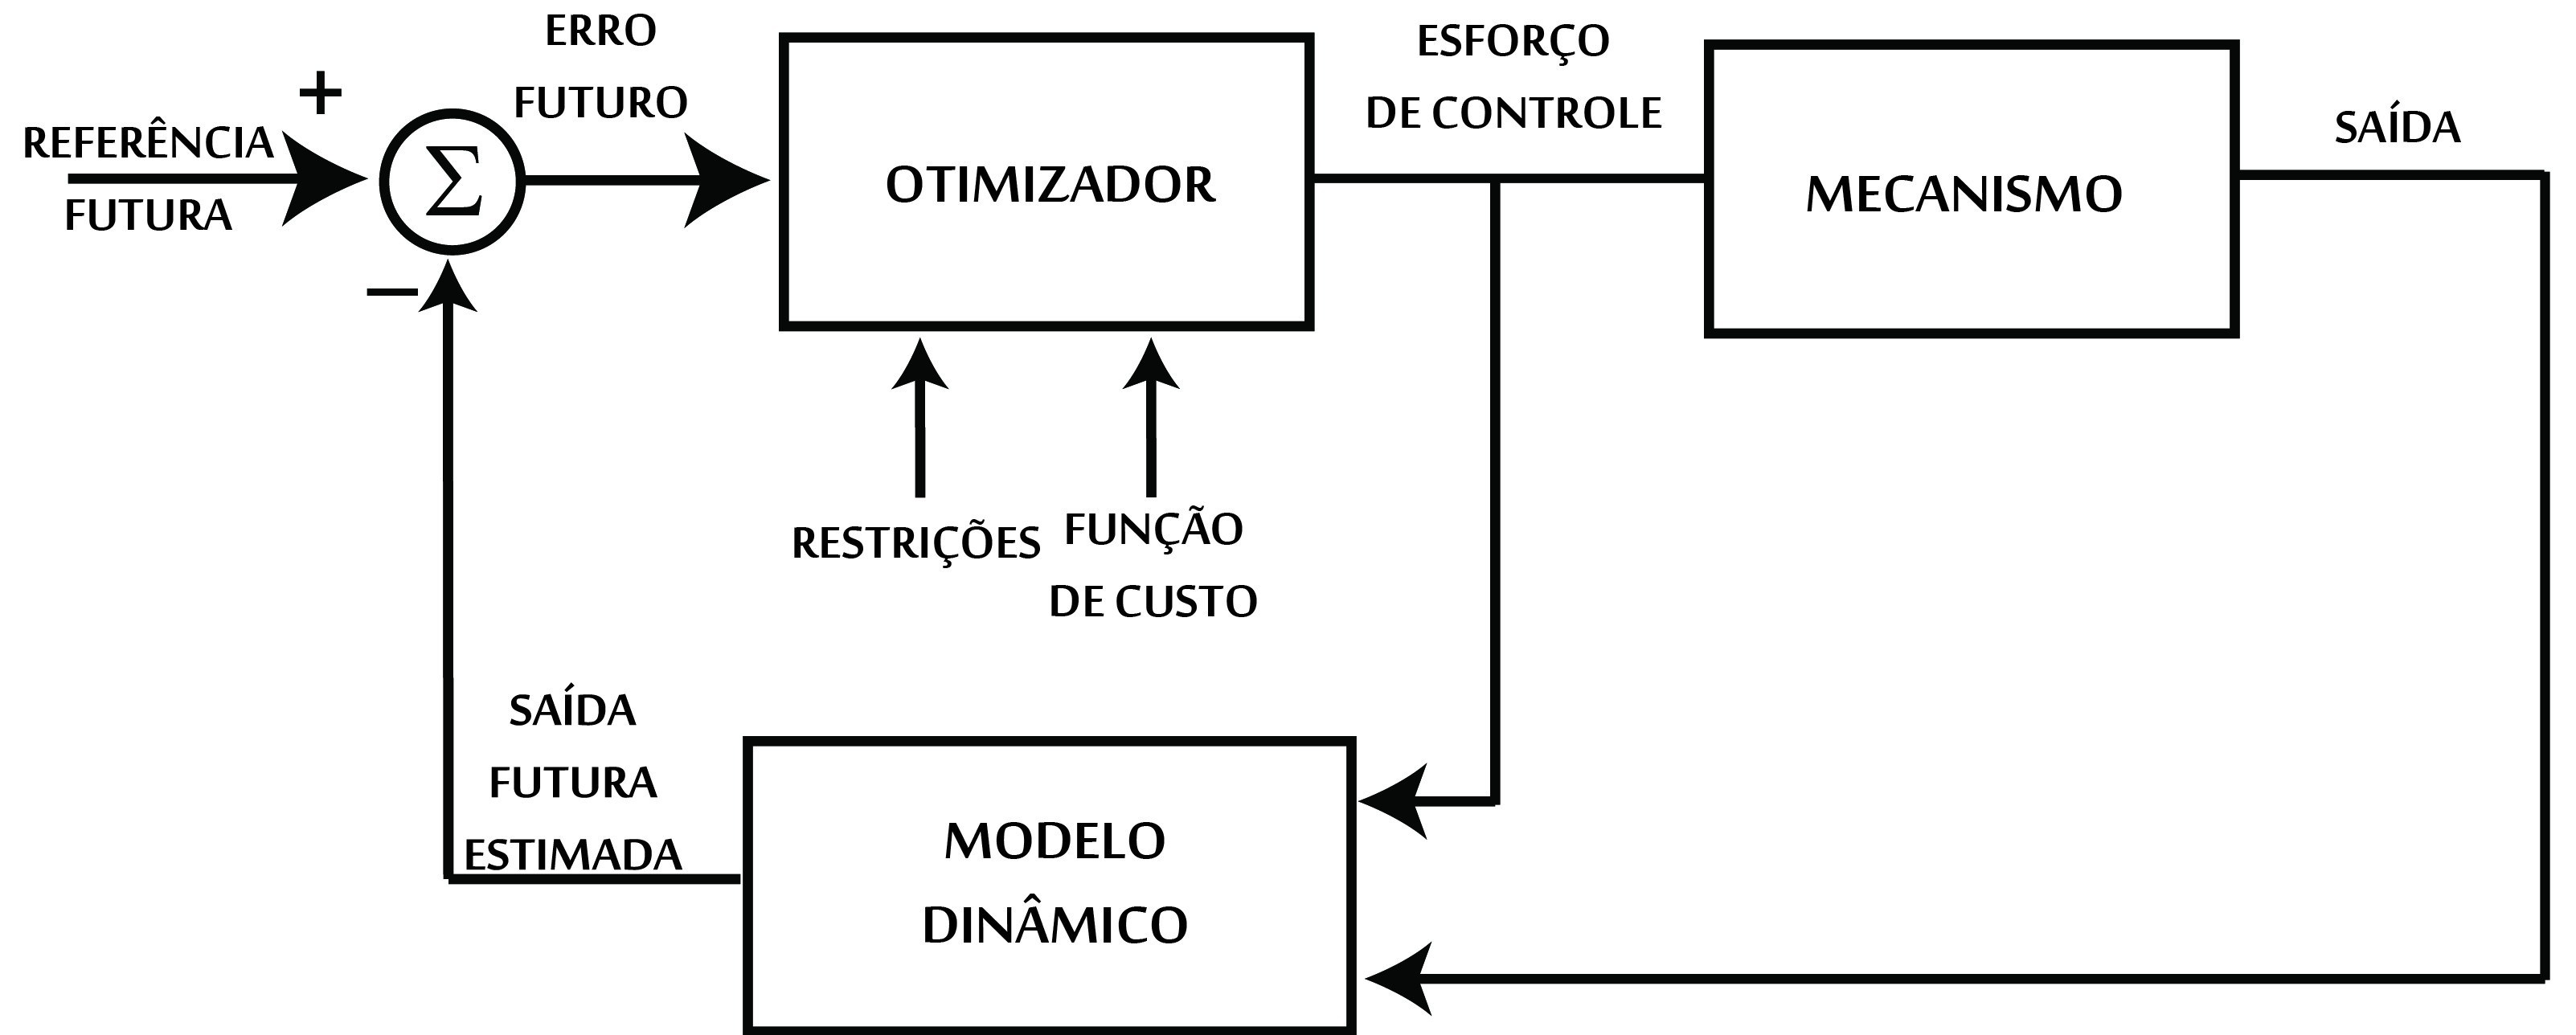
\includegraphics[scale=0.10]{CPM.jpg}
    \end{figure}  
\end{frame}

\begin{frame}{Revisão da Literatura}
    \framesubtitle{Controle}
    \begin{block}{Controle Adaptativo (CA)}
        \begin{itemize}
            \item[$\bullet$] Técnica de controle baseado em modelo \\[8pt]
            \item[$\bullet$] Estimação em tempo real de parâmetros do sistema \\[8pt]
            \item[$\bullet$] Baixa sensibilidade a incertezas paramétricas \\[8pt]
            \item[$\bullet$] Necessita de modelo dinâmico linear em relação aos parâmetros \\[8pt]
            \item[$\bullet$] Alternativamente pode realizar a estimação de termos não lineares de compensação dinâmica \\[8pt]
            \item[$\bullet$] Custo computacional adicional relativo a integração das leis de adaptação \\[8pt]
            \item[$\bullet$] Maior complexidade de projeto e implementação \\[8pt]
        \end{itemize}
    \end{block}
\end{frame}

\begin{frame}{Revisão da Literatura}
    \framesubtitle{Controle}
    \begin{figure}[!h]
        \centering
        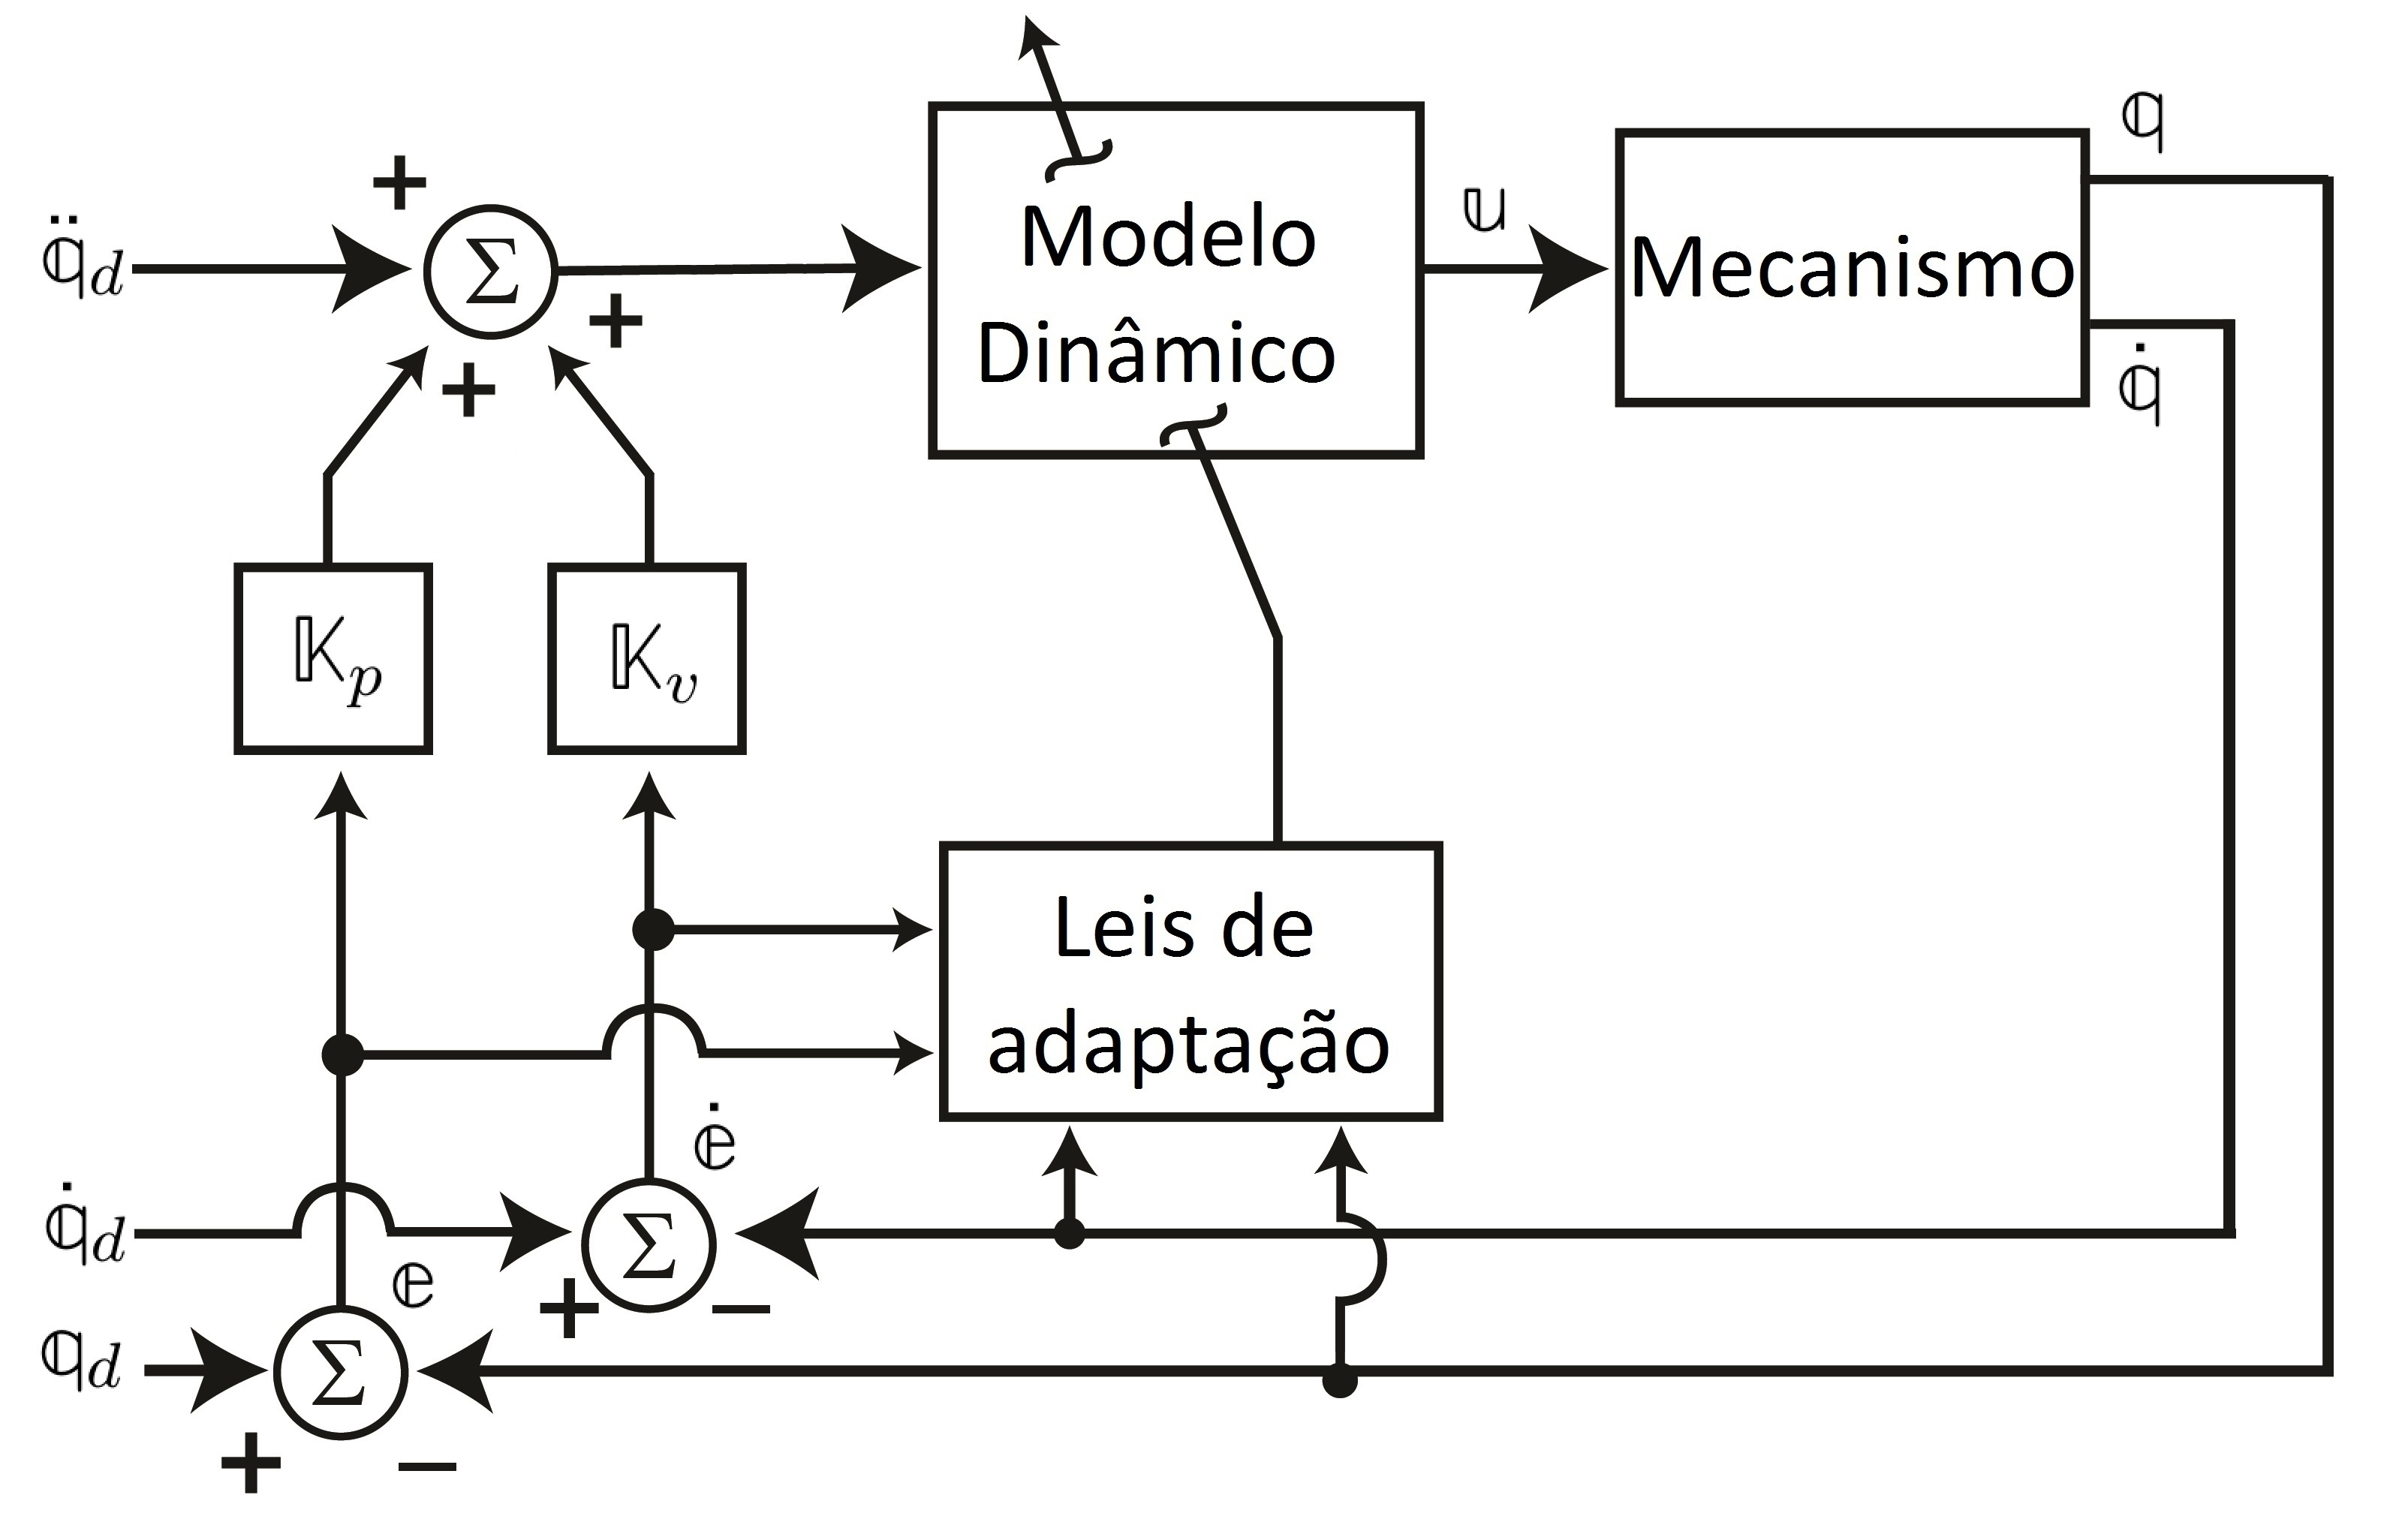
\includegraphics[scale=0.30]{CA.jpg}
    \end{figure}  
\end{frame}

\begin{frame}{Revisão da Literatura}
    \framesubtitle{Controle}
    \begin{block}{Controle por Modos Deslizantes (CMD)}
        \begin{itemize}
            \item[$\bullet$] Técnica de controle não linear robusto \\[8pt]
            \item[$\bullet$] Alta robustez em relação a incertezas estruturadas e não estuturadas \\[8pt]
            \item[$\bullet$] Desempenho menos dependente da qualidade do modelo dinâmico \\[8pt]
            \item[$\bullet$] Utiliza funções descontínuas na lei de controle, o que pode causar \emph{chattering} \\[8pt]
            \item[$\bullet$] Bastante utilizado em combinação com lógica \emph{fuzzy} e redes neurais (Begon \emph{et al.}, 1995; Ertugrul e Kaynak, 2000; Hu e Woo, 2006; Sadati e Ghadami, 2008) \\[8pt]
        \end{itemize}
    \end{block}
\end{frame}

\begin{frame}{Revisão da Literatura}
    \framesubtitle{Controle}
    \begin{figure}[!h]
        \centering
        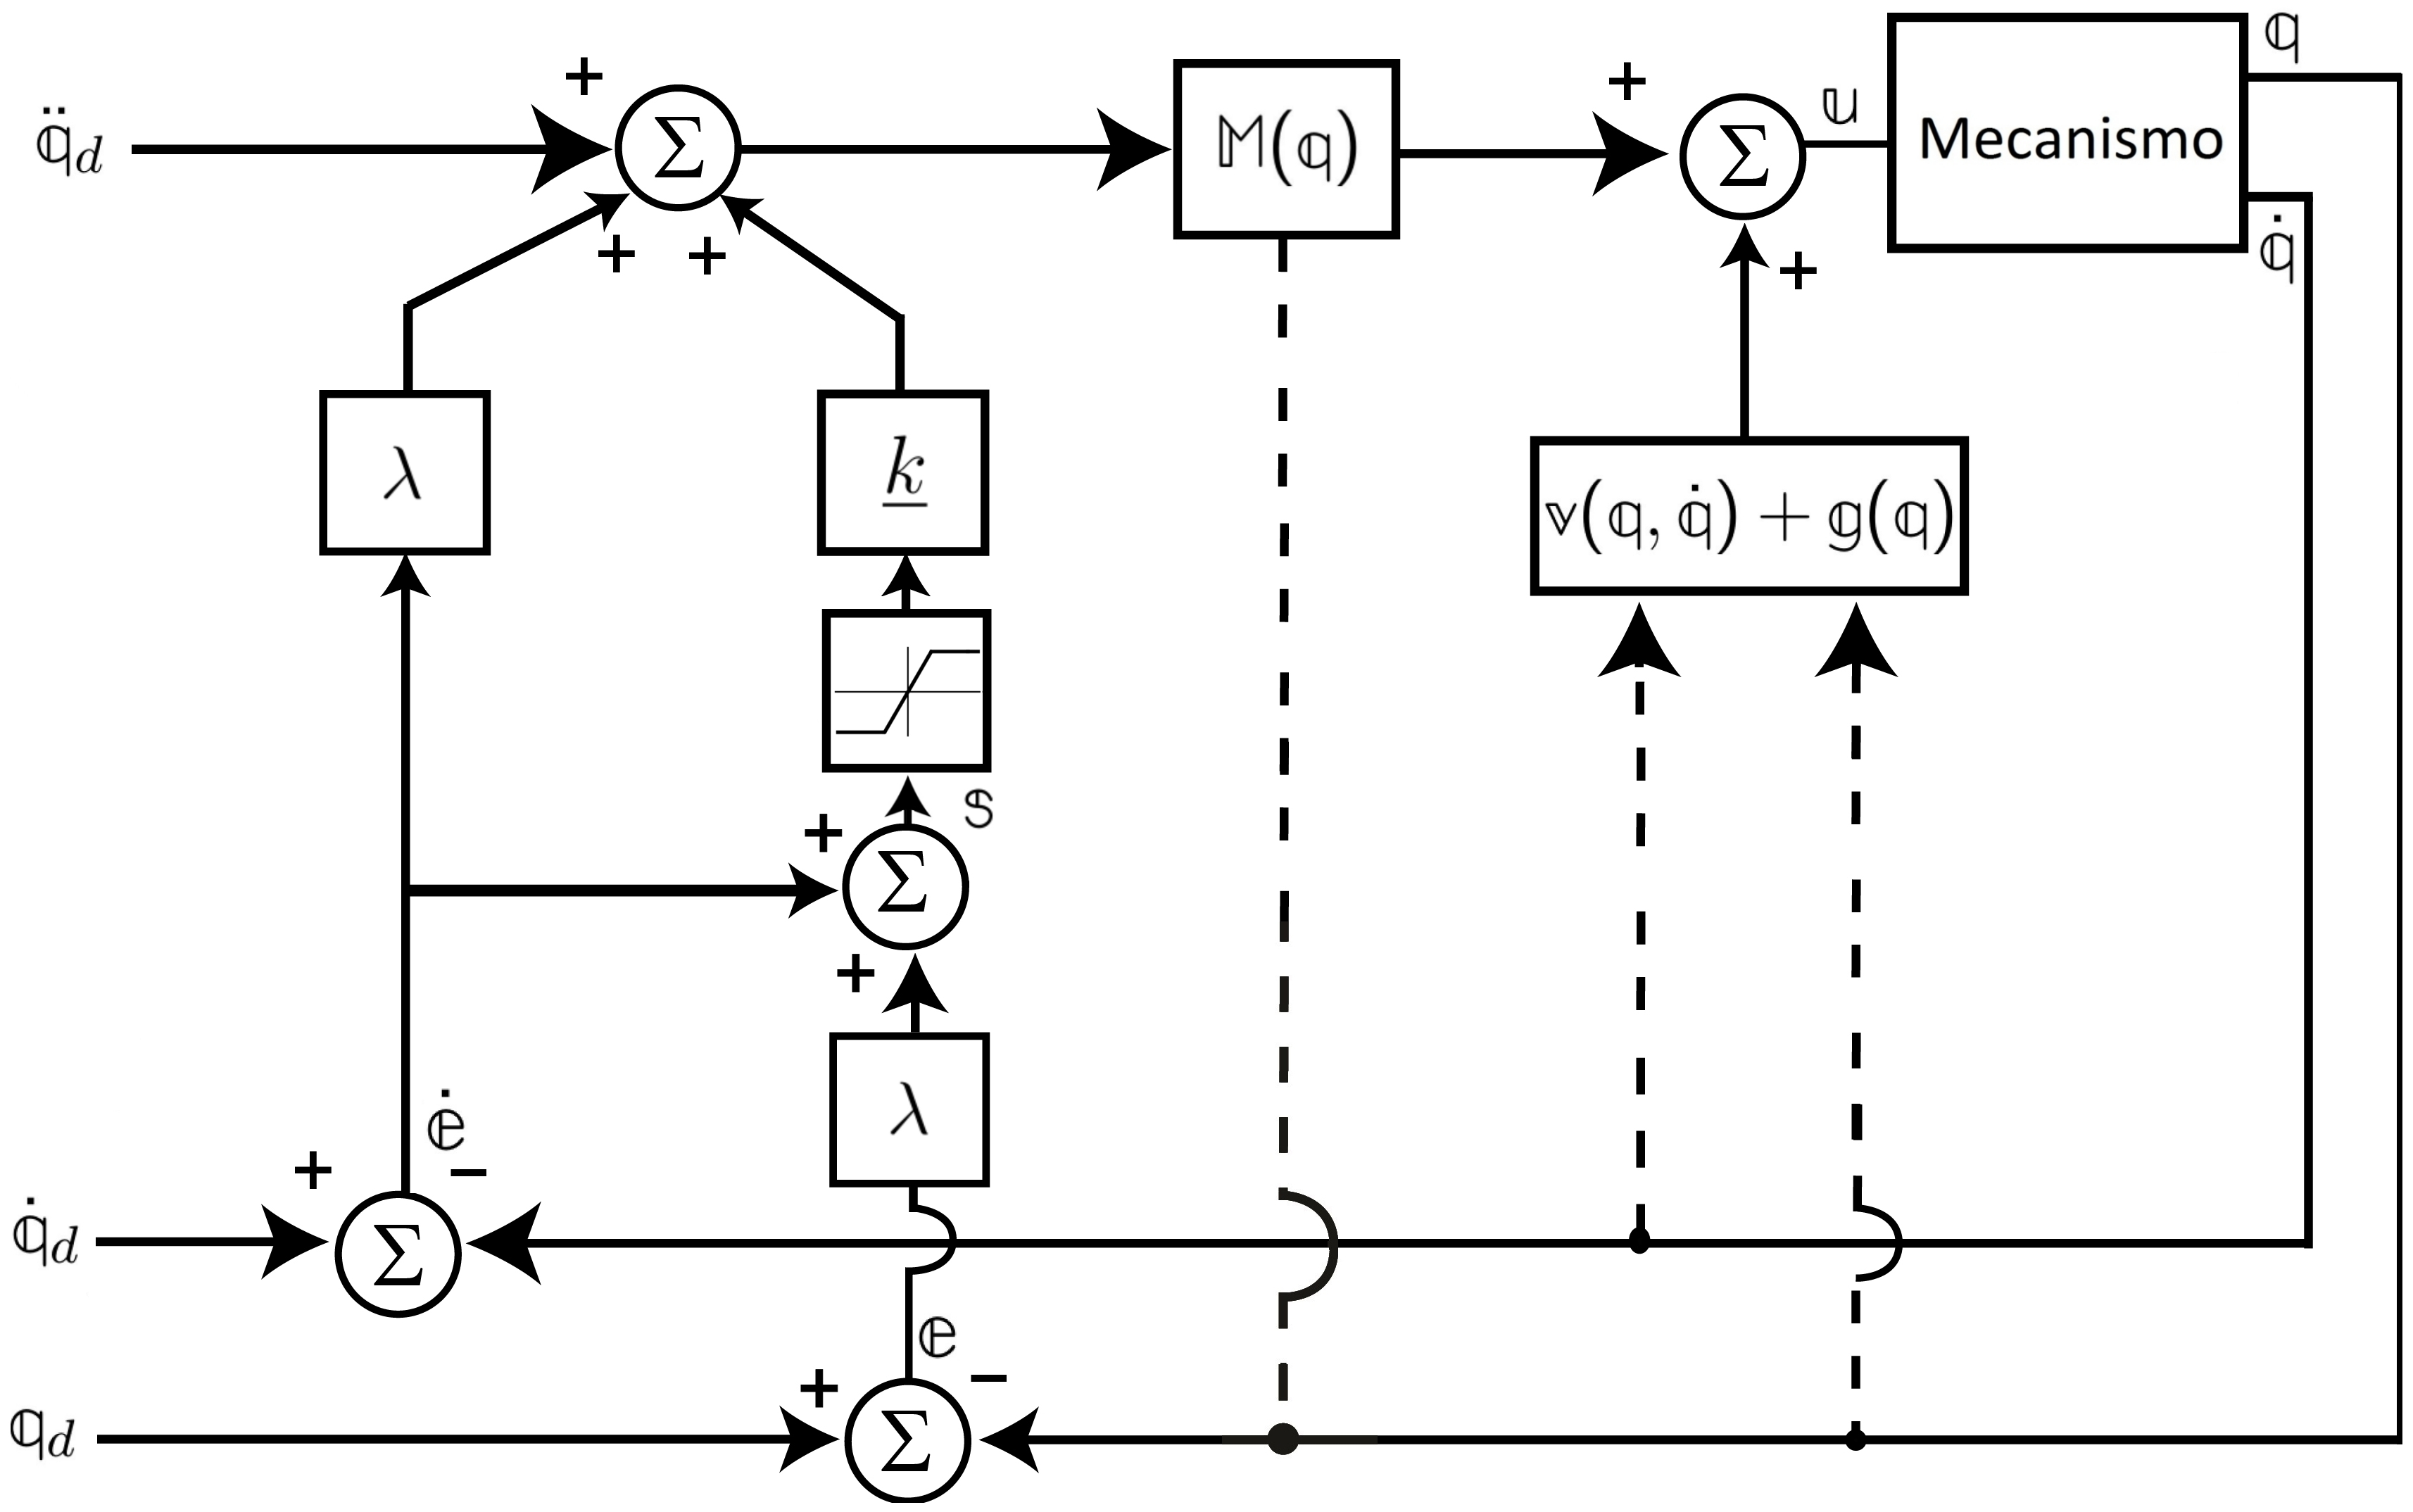
\includegraphics[scale=0.35]{CMD.jpg}
    \end{figure}  
\end{frame}

\begin{frame}{Revisão da Literatura}
    \framesubtitle{Controle}
    \begin{block}{Técnicas de controle combinadas}
        \begin{itemize}
            \item[$\bullet$] "PD-SMC" (Ouyang, Acob, Pano, 2014)
            \begin{itemize}
            	\item[--] Lei de controle combinada não baseada em modelo
            	\item[--] Simulação
            	\item[--] Mecanismo serial prismático (PPP)
            \end{itemize}
            \item[$\bullet$] "PD-SMC" (Li, Ghasemi, Xie, Gao, 2018)
            \begin{itemize}
            	\item[--] Lei de controle combinada não baseada em modelo
            	\item[--] Experimento (movimento lento, trajetória de 150s, controle por câmera)
            	\item[--] Mecanismo serial de 6 gl
            \end{itemize}
            \item[$\bullet$] "Hybrid PD-SMC" (Acob, 2015)
            \begin{itemize}
            	\item[--] Lei de controle combinada não baseada em modelo
            	\item[--] Simulação
            	\item[--] Mecanismo serial de 3 gl e mecanismo paralelo de 2 gl
            \end{itemize}
        \end{itemize}
    \end{block}
\end{frame}

\begin{frame}{Revisão da Literatura}
    \framesubtitle{Controle}
    \begin{block}{Técnicas de controle combinadas}
        \begin{itemize}
            \item[$\bullet$] "PD-SMC-GA" (Mahmoodabadi, Taherkhorsandi, Talebipour, Castilho-Villar, 2015)
            \begin{itemize}
            	\item[--] Lei de controle combinada baseada em modelo
            	\item[--] Simulação
            	\item[--] Pêndulo invertido
            \end{itemize}
        \item[$\bullet$] "NN-SMC" (Truong, Tran, Ahn, 2019)
            \begin{itemize}
            	\item[--] Lei de controle baseada em modelo
            	\item[--] Experimento (movimento lento, ciclo de 10s)
            	\item[--] Mecanismo serial hidráulico de 3 gl
            	\item[--] Rede neural realiza a sintonização em tempo real dos ganho do controlador
            \end{itemize}
        \end{itemize}
    \end{block}
    $$ $$
    $$ $$
\end{frame}

\begin{frame}{Metodologia da Pesquisa}
	\pause
    \begin{block}{Modelagem}
        Desenvolvimento e implementação de algoritmo genérico para modelagem dinâmica de mecanismos paralelos translacionais
    \end{block}
    \pause
    \begin{block}{Controle}
        Estudo, síntese, e simulação de leis de controle não linear robusto de alto desempenho para mecanismos paralelos 
    \end{block}
    \pause
    \begin{block}{Experimento}
		Contrução de um protótipo de manipulador paralelo translacional e realização de ensaios experimentais com o intuito de:
		\begin{itemize}
			\item[--] Validar a eficácia da utilização do modelo gerado pelo algoritmo em leis de controle baseadas em modelo
			\item[--] Comparar o desempenho das leis de controle propostas com leis de controle já consagradas pela literatura
		\end{itemize}
    \end{block}
\end{frame}

\begin{frame}{Algoritmo de Modelagem}
    \framesubtitle{Cadeias seriais}
	\begin{figure}[!h]
        \centering
        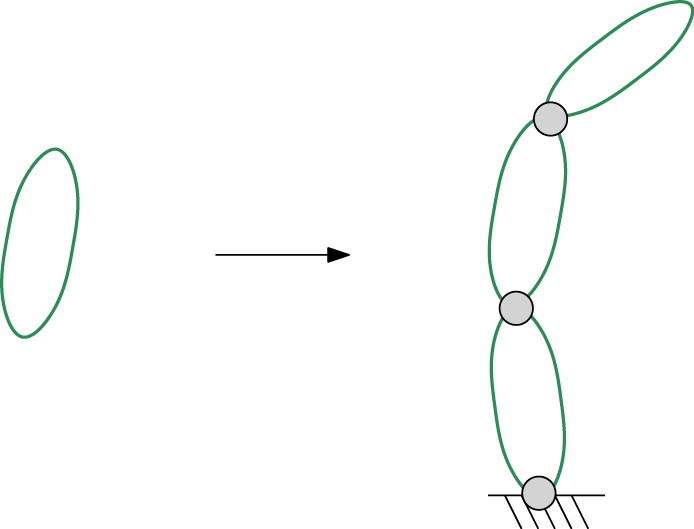
\includegraphics[scale=1.00]{Elo2Serial.jpg}
    \end{figure} 
\end{frame}

\begin{frame}{Algoritmo de Modelagem}
    \framesubtitle{Cadeias seriais}
    \begin{block}{Elementos}
		\begin{itemize}
			\item[--] Elos
			\item[--] Juntas
			\item[--] Atuadores
		\end{itemize}
    \end{block}
	\pause
    \begin{block}{Descrição Topológica}
		\begin{itemize}
			\item[--] Parâmetros de Denavit-Hartenberg
			\item[--] Coordenadas dos centros de massa dos elos nos sistemas móveis
		\end{itemize}
    \end{block}
	\pause
    \begin{block}{Efeitos considerados}
		\begin{itemize}
			\item[--] Ação da gravidade
			\item[--] Inércia distribuída
			\item[--] Atritos
			\item[--] Esforço e dinâmica dos atuadores
		\end{itemize}
    \end{block}
\end{frame}

\begin{frame}{Algoritmo de Modelagem}
    \framesubtitle{Manipulador paralelo}
	\begin{figure}[!h]
        \centering
        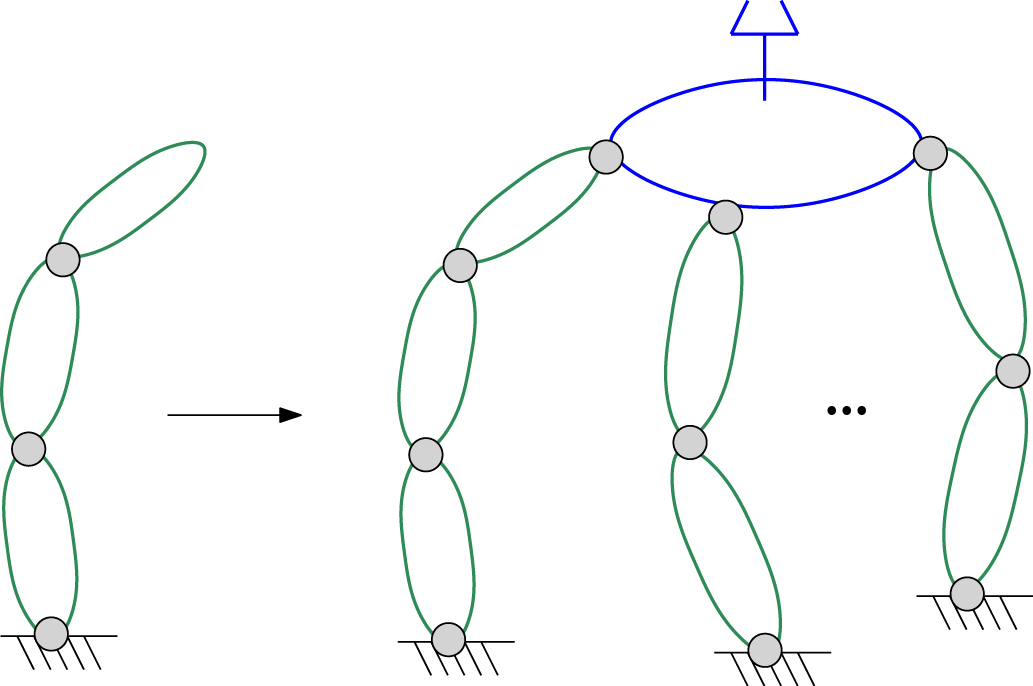
\includegraphics[scale=1.00]{Serial2Paralelo.jpg}
    \end{figure} 
\end{frame}

\begin{frame}{Algoritmo de Modelagem}
    \framesubtitle{Manipulador paralelo}
    \begin{block}{Efetuador}
		\begin{itemize}
			\item[--] Subsistema $\ssB_0$
			\item[--] Sistema de coordenadas móvel $\ttB$
			\item[--] Sistema de coordenadas fixo $\ttN_0$
		\end{itemize}
    \end{block}
	\pause
    \begin{block}{Cadeias seriais}
		\begin{itemize}
			\item[--] Subsistemas $\ssB_1, \ssB_2,...,\ssB_n$
			\item[--] Sistemas de coordenadas fixos $\ttN_1, \ttN_2,...,\ttN_n$
		\end{itemize}
    \end{block}
	\pause
    \begin{block}{Coordenadas generalizadas}
		\begin{itemize}
			\item[--] $\mq^*$ ou $\mq_0$: Coordenadas $x,y,z$ do CM do efetuador $\ssB_0$ no sistema $\ttN_0$
			\item[--] $\mq_i$: Deslocamentos relativos das juntas da cadeia $\ssB_i, \; i=1,...,n$
			\item[--] $\mq^\diamond$: Concatenação de todos $\mq_i, \; i=1,...,n$
			\item[--] $\mq$: Concatenação de $\mq^*$ com $\mq^\diamond$
		\end{itemize}
    \end{block}
\end{frame}

\begin{frame}{Algoritmo de Modelagem}
    \framesubtitle{Manipulador paralelo}
    \begin{block}{Cinemática das cadeias seriais}
		\begin{itemize}
			\item[--] $\mx_i(\mq_i)$: Coordenadas $x,y,z$ do efetuador de $\ssB_i$ no sistema $\ttN_i$
			\item[--] $\mv_i(\mq_i, \dot{\mq}_i)$: Velocidade linear do efetuador de $\ssB_i$ no sistema $\ttN_i$
			\item[--] $\ma_i(\mq_i, \dot{\mq}_i, \ddot{\mq}_i)$: Aceleração linear do efetuador de $\ssB_i$ no sistema $\ttN_i$
			\item[--] $\momega_i(\mq_i, \dot{\mq}_i)$: Velocidade angular do efetuador de $\ssB_i$ no sistema $\ttN_i$
			\item[--] $\dot{\momega}_i(\mq_i, \dot{\mq}_i, \ddot{\mq}_i)$: Aceleração angular do efetuador de $\ssB_i$ no sistema $\ttN_i$
			\\[12pt]
%			\item[--] $\mx(\mq^\diamond)$: Concatenação de todos $\mx_i(\mq_i)$
%			\item[--] $\mv(\mq^\diamond, \dot{\mq}^\diamond)$: Concatenação de todos $\mv_i(\mq_i, \dot{\mq}_i)$
%			\item[--] $\ma(\mq^\diamond, \dot{\mq}^\diamond, \ddot{\mq}^\diamond)$: Concatenação de todos $\ma_i(\mq_i, \dot{\mq}_i, \dot{\mq}_i)$
%			\item[--] $\momega(\mq^\diamond, \dot{\mq}^\diamond)$: Concatenação de todos $\momega_i(\mq_i, \dot{\mq}_i)$
%			\item[--] $\dot{\momega}(\mq^\diamond, \dot{\mq}^\diamond, \ddot{\mq}^\diamond)$: Concatenação de todos $\dot{\momega}_i(\mq_i, \dot{\mq}_i, \ddot{\mq}_i)$
		\end{itemize}
		\pause
		$$ \mv(\mq^\diamond, \dot{\mq}^\diamond) = \mJ_{\mathsf{v}}(\mq^\diamond) \cdot \dot{\mq}^\diamond $$
    	$$ \ma(\mq^\diamond, \dot{\mq}^\diamond, \ddot{\mq}^\diamond) = \mJ_{\mathsf{v}}(\mq^\diamond) \cdot \ddot{\mq}^\diamond + \underaccent{\sim}{\ma}(\mq^\diamond, \dot{\mq}^\diamond) $$
    	$$ \momega(\mq^\diamond, \dot{\mq}^\diamond) = \mJ_{\mathsf{w}}(\mq^\diamond) \cdot \dot{\mq}^\diamond $$
    	$$ \dot{\momega}(\mq^\diamond, \dot{\mq}^\diamond, \ddot{\mq}^\diamond) = \mJ_{\mathsf{w}}(\mq^\diamond) \cdot \ddot{\mq}^\diamond + \underaccent{\sim}{\dot{\momega}}(\mq^\diamond, \dot{\mq}^\diamond) $$
    \end{block}
\end{frame}

\begin{frame}{Algoritmo de Modelagem}
    \framesubtitle{Manipulador paralelo}
    \begin{block}{Vínculos de posição}
    	Vinculando o efetuador de cada cadeia $\ssB_i$ ao efetuador $\ssB_0$:
    	\begin{equation} \tag{5.13}
    		\mq^* = \md_i + \mE_i \, \mx_i(\mq_i), \; i=1,...,n
    	\end{equation}
    	$$ \md_i = \vct{\tto_i}_{\ttN_0} - \vct{\boldsymbol{1}}_{\ttN_0 \rl \ttB} \vct{\ttp_i}_{\ttB}  $$
    \end{block}
    \begin{figure}[!h]
        \centering
        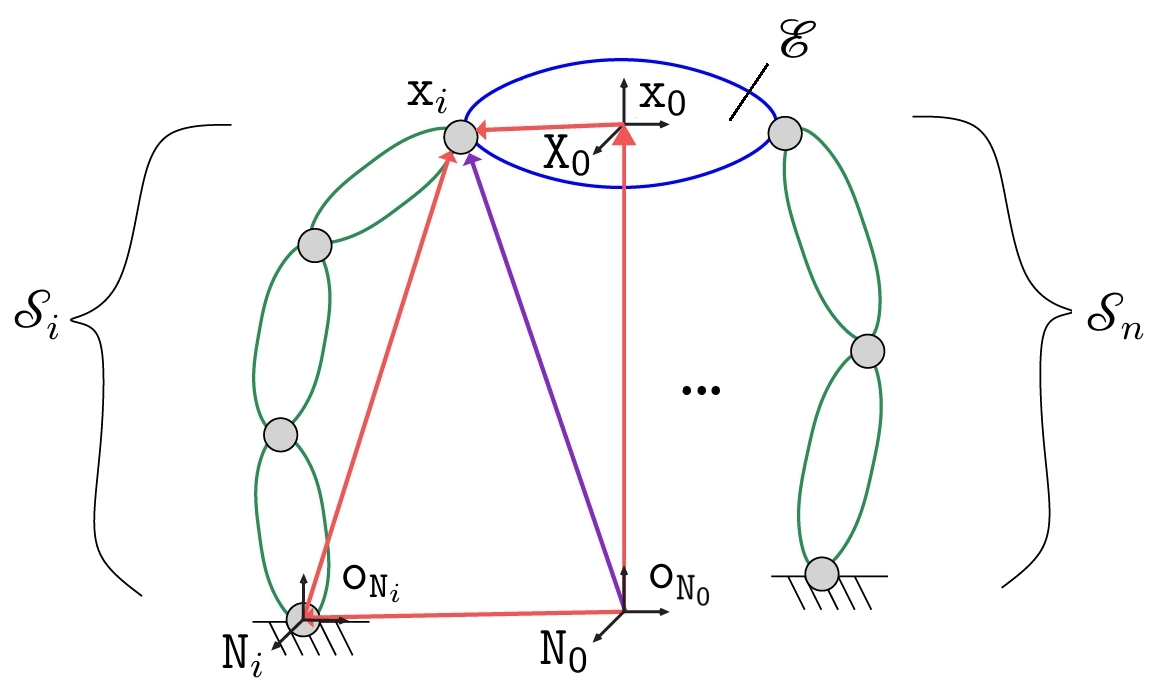
\includegraphics[scale=0.60]{VinculosDePosicao.jpg}
    \end{figure}  
\end{frame}

\begin{frame}{Algoritmo de Modelagem}
    \framesubtitle{Manipulador paralelo}
    \begin{block}{Vínculos de posição}
    	Definindo vínculos afins adicionais (se necessário):
    	\begin{equation} \label{eq:VinculosPosicaoAfins} \tag{5.15}
			\mD_{\oplus}\cdot\mq^\ast = \md_{\oplus} + \mF_{\oplus}\cdot\mq^\diamond
		\end{equation}
		\pause
    	Juntando todas as equações vinculares obtidas:
		\begin{equation} \label{eq:VinculosPosicao2} \tag{5.16}
			\begin{bmatrix}
				\mone\\
				\vdots\\
				\mone \\
				\mD_{\oplus}
			\end{bmatrix}
			\cdot
			\mq^\ast =
			\begin{bmatrix}
				\md_1 \\
				\vdots \\
				\md_n \\
				\md_{\oplus}
			\end{bmatrix}
			+
			\begin{bmatrix}
				\mE_1 & \ldots & \mzr\\
				\vdots & \ddots & \vdots\\
				\mzr &\ldots  & \mE_{n} \\
				\mzr &\ldots  & \mzr
			\end{bmatrix}
			\cdot
			\begin{bmatrix}
				\mx_1(\mq_1) \\
				\vdots \\
				\mx_n(\mq_n)
			\end{bmatrix}
			+
			\begin{bmatrix}
				\mzr\\
				\vdots\\
				\mzr \\
				\mF_{\oplus}
			\end{bmatrix}
			\cdot
			\mq^\diamond
		\end{equation}
	\pause
	Assim, temos:
	\begin{equation} \label{eq:VinculosGenericosPosicao} \tag{5.17}
		\therefore \overline{\mq}(\mq) = \mD \cdot \mq^\ast - \md - \mE \cdot \mx(\mq)
		- \mF \cdot \mq^\diamond = \mzr
	\end{equation}
    \end{block}
\end{frame}

\begin{frame}{Algoritmo de Modelagem}
    \framesubtitle{Manipulador paralelo}
    \begin{block}{Vínculos de quasi-velocidades}
		\begin{equation} \label{eq:VinculosQuasiVel} \tag{5.32}
			\overline{\mp}(\mq,\dot{\mq}) = 
			\begin{bmatrix}
				\dot{\overline{\mq}}(\mq,\dot{\mq}) \\
				\overline{\momega}(\mq,\dot{\mq})
			\end{bmatrix}
			= 
			\begin{bmatrix}
				\mD \cdot \dot{\mq}^\ast  - \mE \cdot \mJ_{\mathsf{v}}(\mq^\diamond) \cdot \dot{\mq}^\diamond  - \mF \cdot \dot{\mq}^\diamond \\
				 - \mQ \cdot \mJ_{\mathsf{w}}(\mq^\diamond) \cdot \dot{\mq}^\diamond
			\end{bmatrix}
			=
			\mzr
		\end{equation}

		\pause
		\begin{equation} \label{eq:VinculosQuasiVel2} \tag{5.34}
			\therefore \overline{\mp}(\mq,\dot{\mq}) = \mA(\mq) \dot{\mq} = \mzr
		\end{equation}
		Sendo
		\begin{equation} \tag{5.35}
			\mA(\mq) = 
			\begin{bmatrix}
				\mD  & -(\mE \cdot \mJ_{\mathsf{v}}(\mq^\diamond) + \mF) \\
				\mzr & -\mQ \cdot \mJ_{\mathsf{w}}(\mq^\diamond) \\
			\end{bmatrix}
		\end{equation}
    \end{block}
\end{frame}

\begin{frame}{Algoritmo de Modelagem}
    \framesubtitle{Manipulador paralelo}
    \begin{block}{Vínculos de quasi-acelerações}
		\begin{equation} \label{eq:VinculosQuasiAce} \tag{5.36}
		\begin{split}
			\dot{\overline{\mp}}(\mq,\dot{\mq},\ddot{\mq}) =
			\begin{bmatrix}
				\ddot{\overline{\mq}}(\mq,\dot{\mq},\ddot{\mq}) \\
				\dot{\overline{\momega}}(\mq,\dot{\mq},\ddot{\mq})
			\end{bmatrix}
			= 
			\begin{bmatrix}
				\mD \cdot \ddot{\mq}^\ast - \mE \cdot (\mJ_{\mathsf{v}}(\mq^\diamond) \cdot \ddot{\mq}^\diamond + \underaccent{\sim}{\ma}(\mq, \dot{\mq}))  - \mF \cdot \ddot{\mq}^\diamond \\
				- \mQ \cdot (\mJ_{\mathsf{w}}(\mq^\diamond) \cdot \ddot{\mq}^\diamond + \underaccent{\sim}{ \dot{\momega} }(\mq, \dot{\mq}))
			\end{bmatrix}
			\\
			= \mzr
		\end{split}
		\end{equation}

		\pause
		\begin{equation} \label{eq:VinculosQuasiAce_} \tag{5.39}
			\therefore \dot{\overline{\mp}}(\mq,\dot{\mq},\ddot{\mq}) = \mA(\mq)\ddot{\mq} + \mb(\mq,\dot{\mq}) = \mzr
		\end{equation}
		Sendo
		\begin{equation} \tag{5.40}
			\mb(\mq,\dot{\mq}) =
			-\begin{bmatrix}
				\mE \cdot \underaccent{\sim}{\ma}(\mq, \dot{\mq}) \\
				\mQ \cdot \underaccent{\sim}{\dot{\momega}}(\mq, \dot{\mq}) \\
			\end{bmatrix}
		\end{equation}
    \end{block}
\end{frame}

\begin{frame}{Algoritmo de Modelagem}
    \framesubtitle{Manipulador paralelo}
    \begin{block}{Modelos dinâmicos desacoplados}
    	\begin{equation} \label{eq:ModeloDosSubsistemas} \tag{5.1}
			\overline{\mf}_{\ssB_i}(\mu_i, \mq_i, \dot{\mq}_i, \ddot{\mq}_i) =  \mu_{\ssB_i} - \Big(\mM_{\ssB_i}(\mq_i) \ddot{\mq}_i + \mnu_{\ssB_i}(\mq_i,\dot{\mq}_i) + \mg_{\ssB_i}(\mq_i)\Big) = \mzr, \, i = 0,...,n
		\end{equation}
    \end{block}
    \pause
    \begin{block}{Princípio de D'Alambert}
    	\begin{equation} \tag{5.48}
			\sum_{i=0}^n \delta W_i = \sum_{i=0}^n \delta \mq_i^\msT \cdot \overline{\mf}_{\ssB_i} = 0
		\end{equation}
		\pause
		Ou seja:
		\begin{equation} \label{eq:DAlambertParalelos} \tag{5.49}
			\delta \mq^\msT \cdot \mf = 0
		\end{equation}
    \end{block}
\end{frame}

\begin{frame}{Algoritmo de Modelagem}
    \framesubtitle{Manipulador paralelo}
    \begin{block}{Vínculos em forma diferencial}
    \pause
    	\begin{equation} \label{eq:Adeltaq} \tag{5.50}
			\mA(\mq) \delta \mq = \mzr
		\end{equation}
	    \pause
		\begin{equation} \label{eq:deltaQsshQcir} \tag{5.52}
			\delta\mq = \mQ\ssh \delta\mq\ssh + \mQ\cir \delta\mq\cir
		\end{equation}
		\pause
		\begin{equation} \label{eq:deltamqC} \tag{5.54}
			\therefore \delta \mq = \mC(\mq) \cdot \delta\mq\ssh
		\end{equation}
		\pause
		Sendo:
		\begin{equation} \label{eq:CComplemento} \tag{5.55}
			\mC(\mq) = \mQ\ssh - \mQ\cir (\mA \mQ\cir)^{-1} \mA \mQ\ssh 
		\end{equation}
    \end{block}
    \pause
    \begin{block}{Equações dinâmicas}
    	\begin{equation} \tag{5.57/5.58}
			\delta {\mq\ssh}^\msT \mC^\msT \mf = 0 \Leftrightarrow \mC^\msT \mf = \mzr
		\end{equation}
    \end{block}
\end{frame}

\begin{frame}{Algoritmo de Modelagem}
    \framesubtitle{Manipulador paralelo}
    \begin{block}{Dinâmica Direta}
    	\pause
    	Sistema de Equações Diferenciais Algébricas
    	\begin{equation*}
			\begin{cases}
			\mC(\mq)^\msT (   \mM'(\mq)\ddot{\mq} + \mnu'(\mq,\dot{\mq}) + \mg'(\mq) ) = \mC(\mq)^\msT \mu' \\
			\bar{\mq}(\mq) = \mzr
			\end{cases}
		\end{equation*}
		\pause
		Sistema de Equações Diferenciais
    	\begin{equation} \tag{5.60}
			\begin{cases}
			\mC(\mq)^\msT (   \mM'(\mq)\ddot{\mq} + \mnu'(\mq,\dot{\mq}) + \mg'(\mq) ) = \mC(\mq)^\msT \mu' \\
			\mA(\mq)\ddot{\mq} + \mb(\mq,\dot{\mq}) = \mzr
			\end{cases}
		\end{equation}
		\pause
		Utilizando o método de estabilização de Baumgarte
		\begin{equation} \tag{5.65}
			\begin{bmatrix}
				\mC(\mq)^\msT \mM'(\mq) \\
				\mA(\mq)
			\end{bmatrix}
			\cdot
			\ddot{\mq}
			=
			\begin{bmatrix}
				\mC(\mq)^\msT (\mu' - \mnu'(\mq,\dot{\mq}) - \mg'(\mq) ) \\
				-\mb(\mq,\dot{\mq}) -
				2\lambda
				\mA(\mq) \cdot \dot{\mq} -
				\lambda^2
				\overline{\mq}(\mq) \\
			\end{bmatrix}
		\end{equation}
    \end{block}
\end{frame}

\begin{frame}{Algoritmo de Modelagem}
    \framesubtitle{Manipulador paralelo}
    \begin{block}{Dinâmica Direta}
    	\pause
    	\begin{equation} \label{eq:DinamicaInversa2} \tag{5.73}
			\mM_{\ssM} (\mq) \ddot{\mq}\ssh + \mnu_{\ssM}(\mq, \dot{\mq}) + \mg_{\ssM}(\mq)   = \mZ(\mq)^{\msT} \mu^\star
		\end{equation}
		\pause
		Sendo: 
		\begin{equation} \tag{5.74}
			\mM_{\ssM}  =  \mC^\msT \mM' \mC
		\end{equation}
		\begin{equation} \tag{5.75}
			\mnu_{\ssM}  =  \mC^\msT (  \mM'  \mc  + \mnu' )
		\end{equation}
		\begin{equation} \tag{5.76}
			\mg_{\ssM}  = \mC^\msT \mg'
		\end{equation}

		\pause
		\begin{equation} \tag{5.68}
			\mc = - (\mA \mQ\cir)^\msI \, \mb
		\end{equation}
		\begin{equation} \tag{5.71*}
			\mZ = \mU^\msT \mC
		\end{equation}
		\begin{equation} \label{eq:u_estrela} \tag{5.69}
			\mu' = \mU \cdot \mu^\star
		\end{equation}
    \end{block}
\end{frame}

\begin{frame}{Controle}
    %\framesubtitle{Manipulador paralelo}
    \pause
    \begin{block}{Modelo}
    	\begin{equation} \label{eq:ModeloControle} \tag{6.4}
			\mH(\mq) \, \ddot{\mq}\ssh + \mh(\mq,\dot{\mq}) = \mup
		\end{equation}
		\pause
		Sendo
		\begin{equation} \tag{6.1}
			\mH(\mq) = \mM_{\ssM}(\mq)
		\end{equation}
		\begin{equation} \tag{6.2}
			\mh(\mq, \dot{\mq}) = \mv_{\ssM}(\mq, \dot{\mq}) + \mg_{\ssM}(\mq)
		\end{equation}
		\begin{equation} \tag{6.3}
			\mup = \mZ(\mq)^{\msT} \mu^\star
		\end{equation}
    \end{block}
\end{frame}

\begin{frame}{Controle}
    \framesubtitle{Modos deslizantes}
    \pause
    \begin{block}{Superfície de escorregamento}
    	\begin{equation*} 
			\sigma: \ms = \underline{\ms}(\mx, \mr) = \mzr
		\end{equation*} \pause
		\begin{equation*}
			\ms = \mzr \Rightarrow \me \rightarrow \mzr
		\end{equation*}
    \end{block}
    \pause
    \begin{block}{Condição de escorregamento}
		\begin{equation} \tag{6.17}
			V(\ms) = \frac{1}{2} \ms^\msT \mW \, \ms
		\end{equation}
		\begin{equation} \label{eq:SlidingCondition} \tag{6.18}
			\frac{\dd}{\dd t} V(\ms)  \leq -   \ms^\msT \underline{\eta} \sign(\ms) 
		\end{equation}
    \end{block}
\end{frame}

\begin{frame}{Controle}
    \framesubtitle{Modos deslizantes}
    \pause
    \begin{block}{Escolha convencional}
    	\begin{equation} \tag{6.14} 
			\ms = \dot{\me} + \underline{\lambda} \me
		\end{equation} 
		\pause
		Para $\mW = \mone$:
		\begin{equation} \tag{6.28*}
			\mup = \hat{\mH}(\ddot{\mq}\ssh_d + \underline{\lambda} \dot{\me} + \underline{k} \sign(\ms) ) + \hat{\mh}
		\end{equation}
		\pause
		\begin{equation} \label{eq:DesigualdadeK2_a1} \tag{6.32}
			(\mone - | \mH^\msI \tilde{\mH}|_{max} ) \cdot \diag(\underline{k})  \geq \diag(\underline{\eta}) + |\mH^\msI \tilde{\mH}|_{max} |\ddot{\mq}\ssh_d + \underline{\lambda} \dot{\me}| + |\mH^\msI\tilde{\mh}|_{max}
		\end{equation}
	$$ $$	
    \end{block}
\end{frame}

\begin{frame}{Controle}
    \framesubtitle{Modos deslizantes}
    \begin{block}{Escolha convencional}
    	\begin{equation} \tag{6.14} 
			\ms = \dot{\me} + \underline{\lambda} \me
		\end{equation}

		Para $\mW = \mH$:
		\begin{equation} \tag{6.35*}
			\mup = \hat{\mH}(\ddot{\mq}\ssh_d + \underline{\lambda} \dot{\me}) + \frac{1}{2}\dot{\hat{\mH}} \, \ms + \hat{\mh} + \underline{k} \sign(\ms)
		\end{equation}
		\pause
		\begin{equation} \label{eq:DesigualdadeK2_a2} \tag{6.39}
			\diag(\underline{k})  \geq \diag(\underline{\eta}) + \frac{1}{2}|\dot{\tilde{\mH}}|_{max} |\ms| + |\tilde{\mH}|_{max} |\ddot{\mq}\ssh_d + \underline{\lambda} \dot{\me}| + |\tilde{\mh}|_{max}
		\end{equation}
    \end{block}
\end{frame}

\begin{frame}{Controle}
    \framesubtitle{Modos deslizantes}
    \pause
    \begin{block}{Nova escolha proposta}
    	\begin{equation} \tag{6.15} 
			\ms = \ddot{\me} + \underline{k}_v \dot{\me} + \underline{k}_p \me
		\end{equation} 
		\pause
		Para $\mW = \mone$:
		\begin{equation} \tag{6.52*}
			\mup = \hat{\mH} \Big(\ddot{\mq}\ssh_d + \underline{k}_v \dot{\me} + \underline{k}_p \me + \int_{0}^t \underline{k} \sign(\ms) \, \dd \tau \Big) + \hat{\mh}
		\end{equation}
		\pause
		\begin{equation} \label{eq:DesigualdadeK2_b1} \tag{6.56}
		\begin{split}
			(\mone - | \mH^\msI \tilde{\mH}|_{max} ) \cdot \diag(\underline{k})  \geq \diag(\underline{\eta}) + |\mH^\msI ( \dot{\mH} \mH^\msI \tilde{\mH} -\dot{\tilde{\mH}}) |_{max} | \mup'' -\msigma|  + \\ |\mH^\msI \tilde{\mH}|_{max}| \dot{\msigma}| + |\mH^\msI \dot{\mH} \mH^\msI  \tilde{\mh}|_{max}+ |\mH^\msI \dot{\tilde{\mh}}|_{max}
		\end{split}
		\end{equation}
    \end{block}
\end{frame}

\begin{frame}{Controle}
    \framesubtitle{Modos deslizantes}
    \begin{block}{Nova escolha proposta}
    	\begin{equation} \tag{6.15} 
			\ms = \ddot{\me} + \underline{k}_v \dot{\me} + \underline{k}_p \me
		\end{equation} 

		Para $\mW = \mH$:
		\begin{equation} \tag{6.59*}
			\mup = \hat{\mH} \Big(\ddot{\mq}\ssh_d + \underline{k}_v \dot{\me} + \underline{k}_p \me + \int_{0}^t \hat{\mH}^\msI \big( \underline{k} \sign(\ms) +  \frac{1}{2}\dot{\hat{\mH}} \, \ms \big) \, \dd \tau \Big) + \hat{\mh}
		\end{equation}
		\pause
		\begin{equation} \label{eq:DesigualdadeK2_b2} \tag{6.63}
		\begin{split}
			\diag(\underline{k})  \geq \diag(\underline{\eta}) + \frac{1}{2}|\dot{\tilde{\mH}}|_{max} |\ms| + |( \dot{\mH} \mH^\msI \tilde{\mH} -\dot{\tilde{\mH}})|_{max} 	|\mup'' - \msigma |  + \\
			|\tilde{\mH}|_{max} |\dot{\msigma}| + |\dot{\mH} \mH^\msI \tilde{\mh}|_{max} + |\dot{\tilde{\mh}}|_{max}
		\end{split}			
		\end{equation}
		$$ $$
    \end{block}
\end{frame}

\begin{frame}{Controle}
    \framesubtitle{Modos deslizantes}
    \begin{block}{Camada limite}
    	\begin{equation*}
    		\sign(\ms) \rightarrow \sat(\ms/\phi)
    	\end{equation*}
    	\begin{equation*}
    		-\phi < s_i < \phi \Rightarrow e_{max} = \phi/k_p
    	\end{equation*}
    \end{block}
    \begin{figure}[!h]
        \centering
        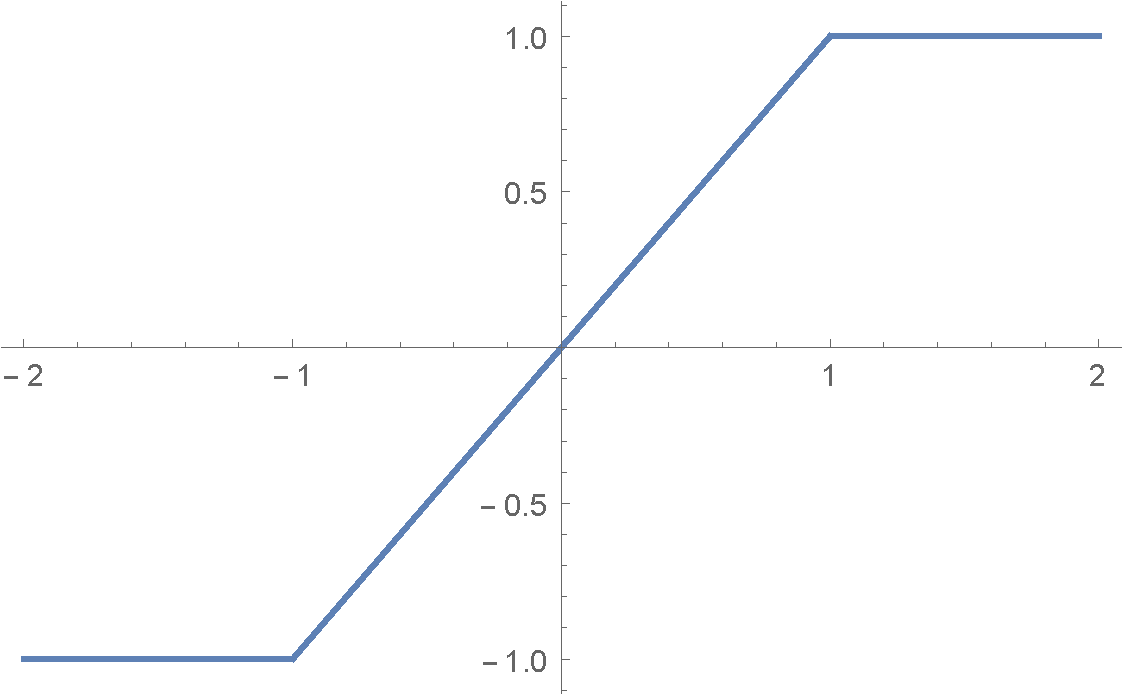
\includegraphics[scale=0.30]{Saturacao.pdf}
    \end{figure}  
\end{frame}

\begin{frame}{Controle}
    \framesubtitle{Modos deslizantes}
    \begin{block}{Lei de Adaptação}
    	\begin{itemize}
    		\item[--] $\underline{k}_i[k+1] = \underline{k}_i[k] + \gamma_i$: Se estiver fora da camada limite e $s_i$ não trocou de sinal 
    		\item[--] $\underline{k}_i[k+1] = \underline{k}_i[k] - \gamma_i$: Se $s_i$ trocou de sinal e $\underline{k}_i[k] \geq \gamma_i$:
    		\item[--] $\underline{k}_i[k+1] = \underline{k}_i[k]$: Caso contrário
    	\end{itemize}
    \end{block}
    \begin{figure}[!h]
        \centering
        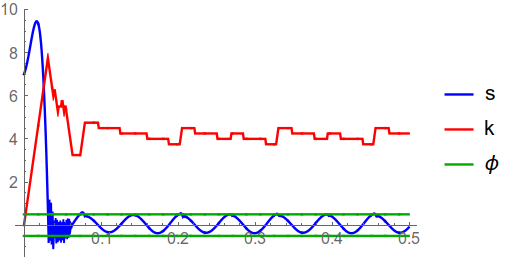
\includegraphics[scale=0.40]{sk.png}
    \end{figure}
\end{frame}

\begin{frame}{Controle}
    \framesubtitle{Modos deslizantes}
    \begin{block}{Lei de controle escolhida}
    	$$ \mup = \hat{\mH}(\mq) \Big( \ddot{\mq}\ssh_d + \underline{k}_v\dot{\me} + \underline{k}_p\me + \int_0^t \underline{k} \, \sat(\ms/\phi) \,\dd \tau \Big) +  \hat{\mh}(\mq, \dot{\mq}) $$
    	Sendo:
    	$$ \ms = \ddot{\me} + \underline{k}_v\dot{\me} + \underline{k}_p\me $$
    \end{block}
    \pause
    \begin{block}{Propriedades}
    	\begin{itemize}
    		\item[--] Robustez característica do CMD
    		\item[--] Grande redução de \emph{chattering} devido à integral
    		\item[--] Similar à lei de CTC (adição de 1 termo)
    		\item[--] Custo computacional muito similar ao do CTC
    	\end{itemize}
    \end{block}
\end{frame}

\begin{frame}{Controle}
    \begin{figure}[!h]
        \centering
        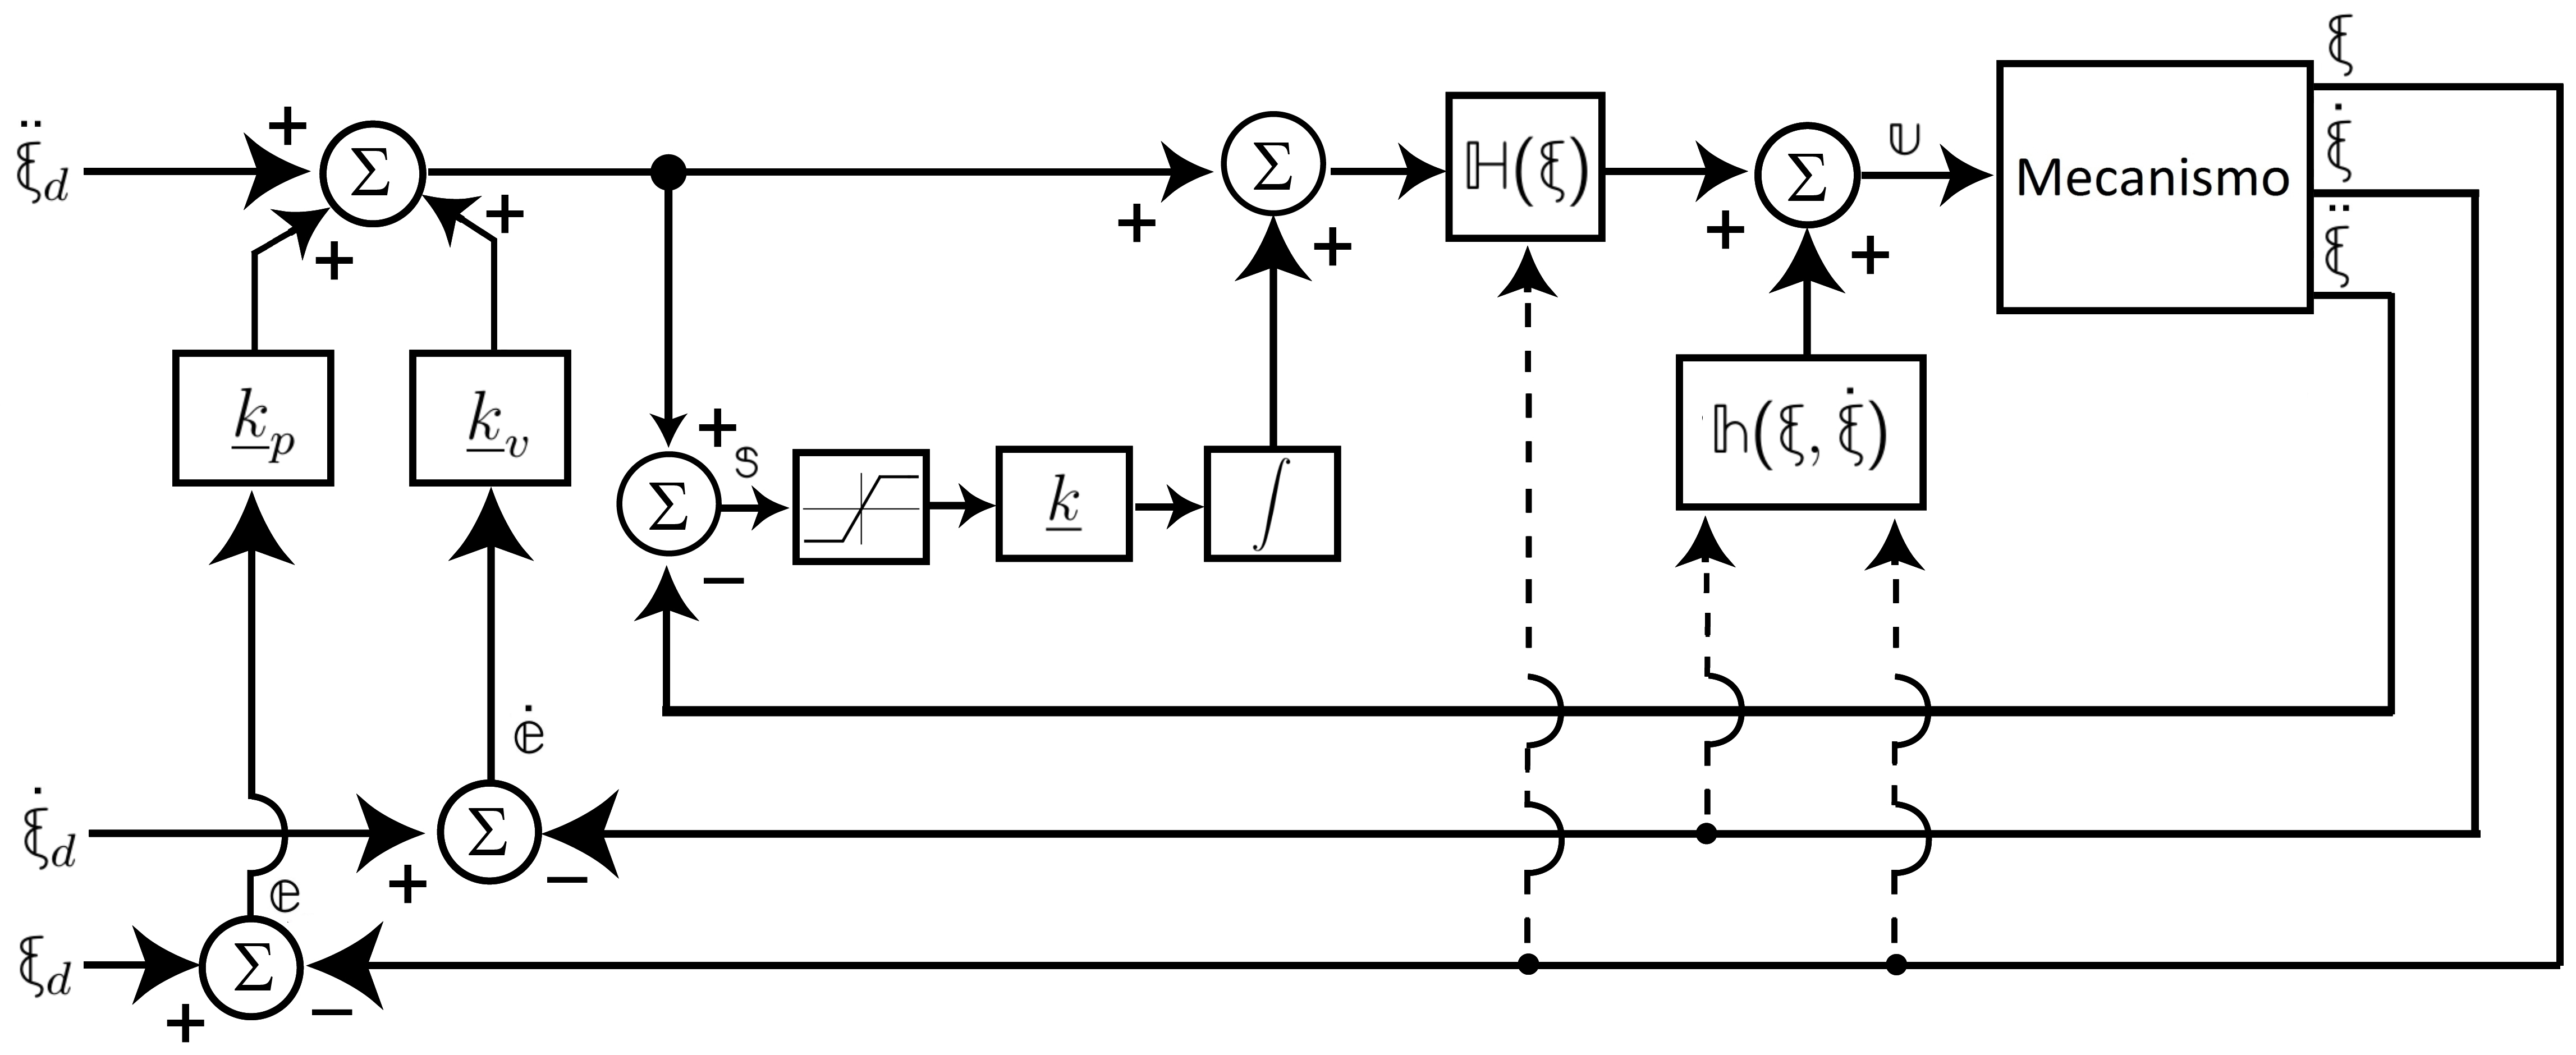
\includegraphics[scale=0.30]{TCMD.jpg}
    \end{figure}
\end{frame}

\begin{frame}{Controle}
    \framesubtitle{Leis utilizadas}
    \begin{block}{PD}
    	$$ \mup = m^* \Big( \ddot{\mq}\ssh_d + \underline{k}_v\dot{\me} + \underline{k}_p\me \Big)$$
    \end{block}
     \pause
    \begin{block}{PDMD}
    	$$ \mup = m^* \Big( \ddot{\mq}\ssh_d + \underline{k}_v\dot{\me} + \underline{k}_p\me + \int_0^t \underline{k} \, \sat(\ms/\phi) \,\dd \tau \Big) $$
    \end{block}
     \pause
    \begin{block}{TC}
    	$$ \mup = \hat{\mH}(\mq) \Big( \ddot{\mq}\ssh_d + \underline{k}_v\dot{\me} + \underline{k}_p\me \Big) +  \hat{\mh}(\mq, \dot{\mq}) $$
    \end{block}
     \pause
    \begin{block}{TCMD}
    	$$ \mup = \hat{\mH}(\mq) \Big( \ddot{\mq}\ssh_d + \underline{k}_v\dot{\me} + \underline{k}_p\me + \int_0^t \underline{k} \, \sat(\ms/\phi) \,\dd \tau \Big) +  \hat{\mh}(\mq, \dot{\mq}) $$
    \end{block}
\end{frame}

\begin{frame}{Experimento}
    \framesubtitle{Bancada Experimental}
    \pause
    \begin{figure}[!h]
        \centering
        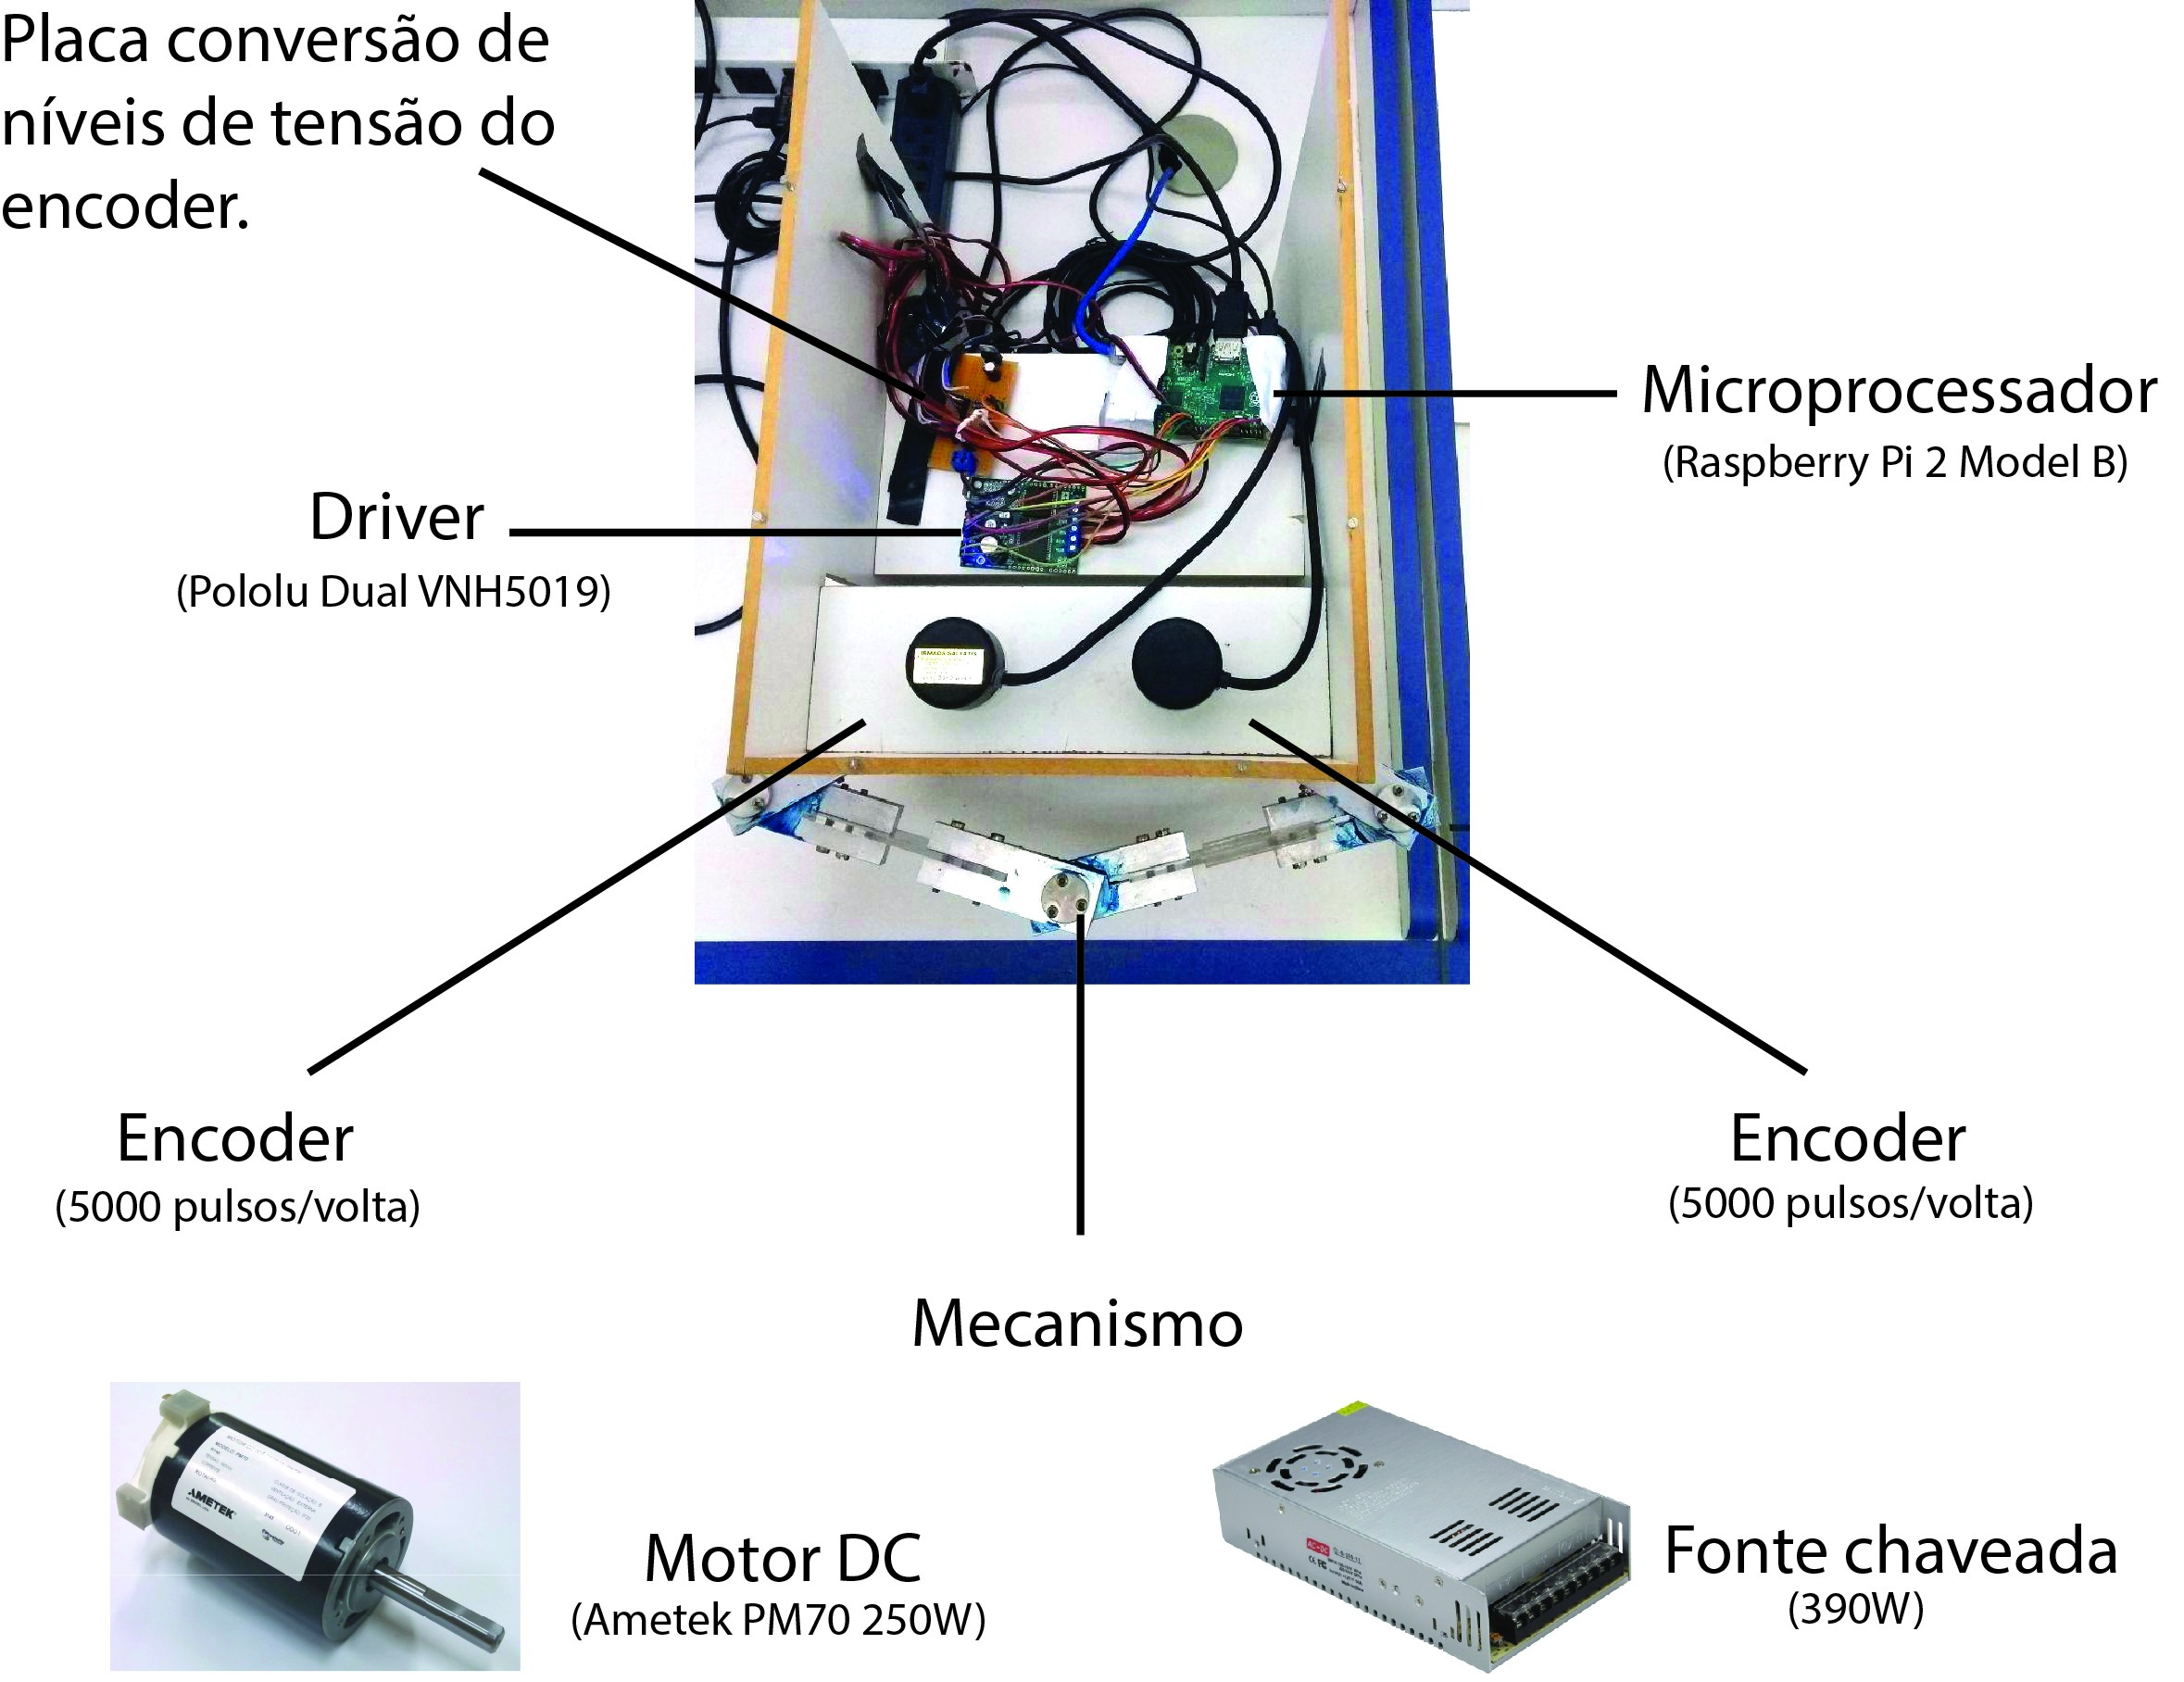
\includegraphics[scale=0.11]{BancadaExperimental.jpg}
    \end{figure}
\end{frame}

\begin{frame}{Experimento}
    \framesubtitle{Bancada Experimental}
    \begin{figure}[!h]
        \centering
        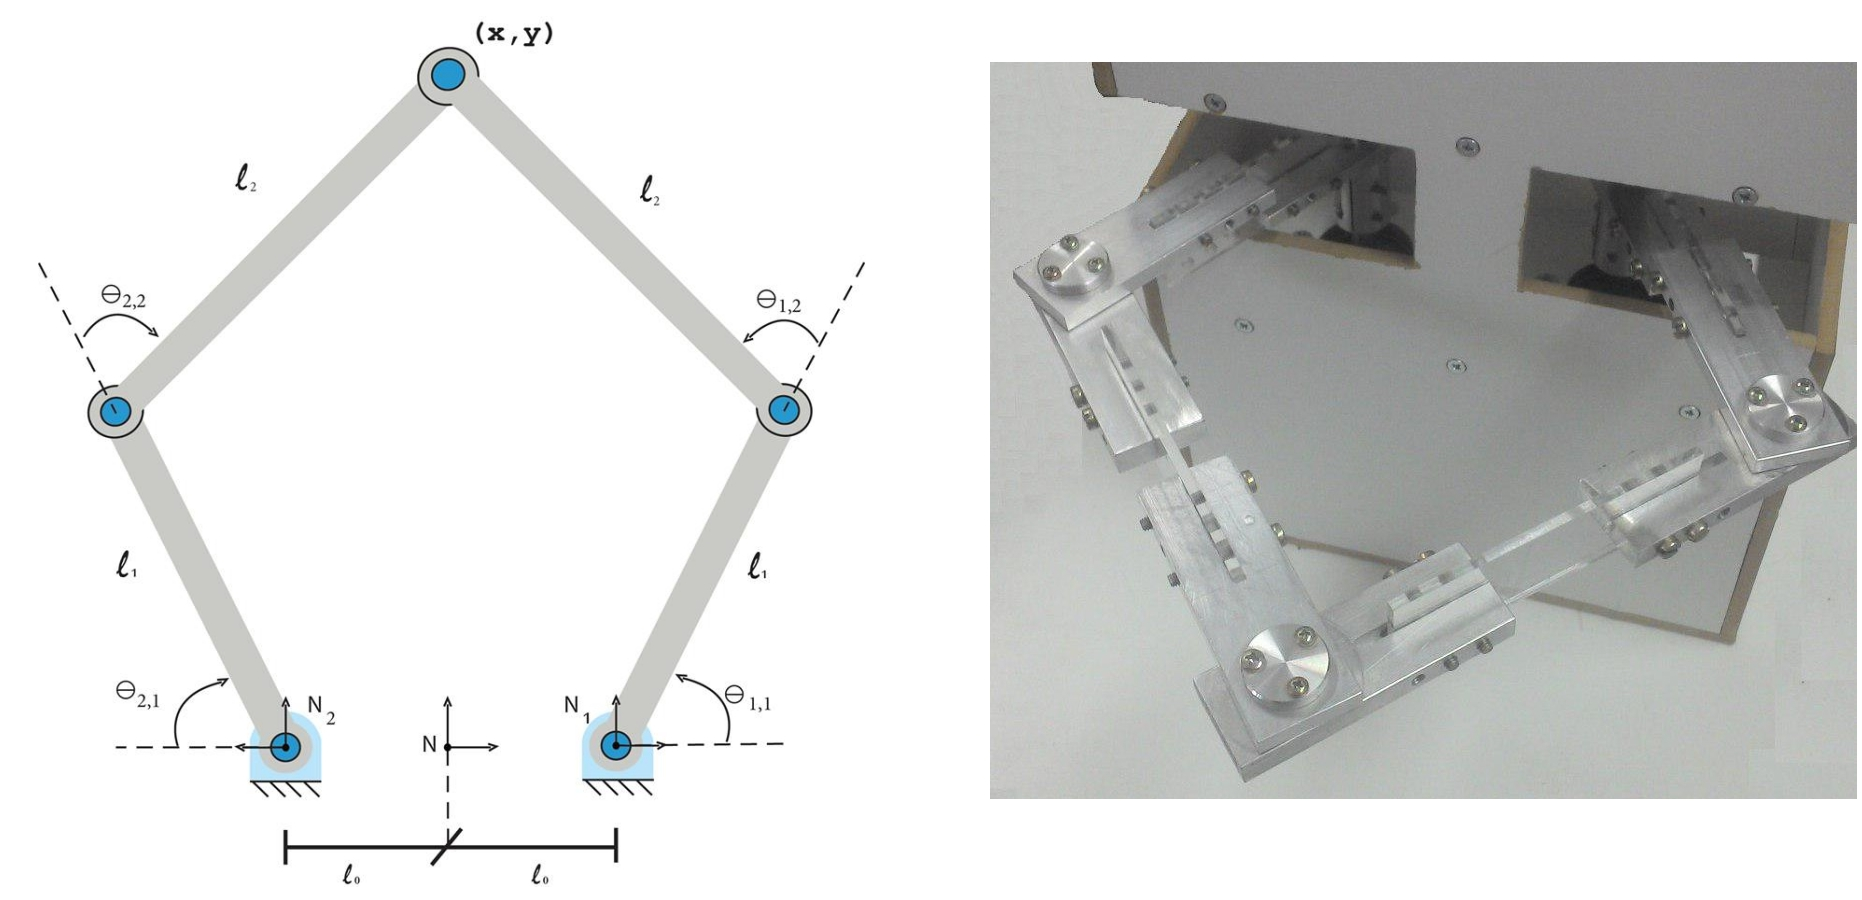
\includegraphics[scale=0.24]{5RscanMec.jpg}
    \end{figure}
\end{frame}

\begin{frame}{Experimento}
    \framesubtitle{Bancada Experimental}
    \begin{figure}[!h]
        \centering
        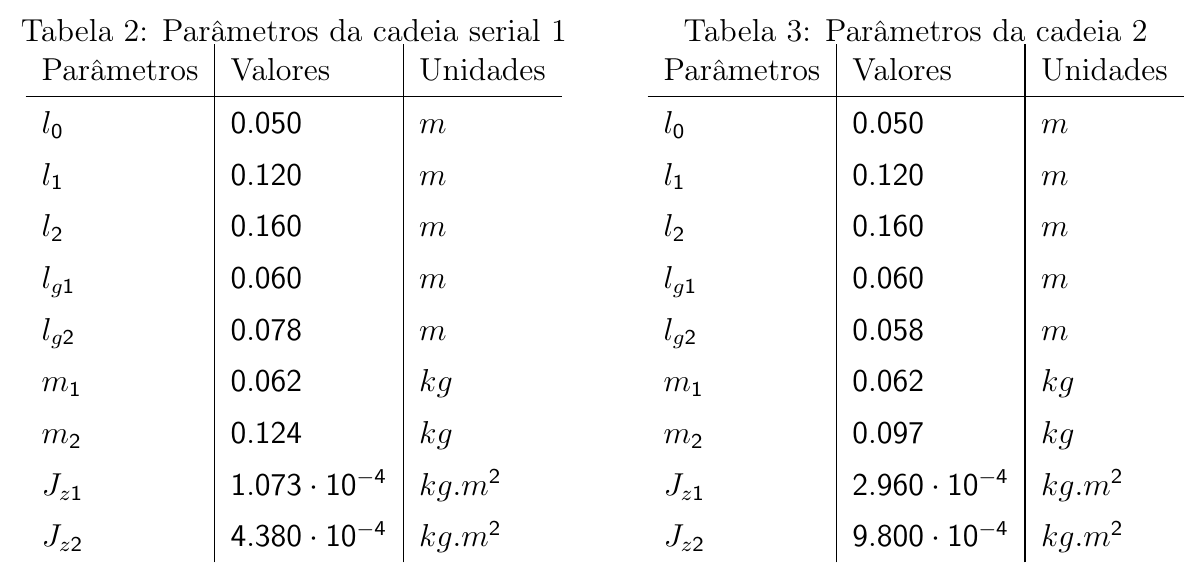
\includegraphics[scale=0.27]{Table.png}
    \end{figure}
\end{frame}

\begin{frame}{Experimento}
    \framesubtitle{PDq - Trejória circular}
	\begin{figure}[!htb]
		\centering
		\subfloat[a)][Trajetória\\ ]{\includegraphics[height=2.8cm,keepaspectratio]{PDq_circulo/xy.png}}
		\subfloat[b)][$e_x$\\ ]{\includegraphics[height=2.8cm,keepaspectratio]{PDq_circulo/ex.png}}
		\subfloat[c)][$e_y$\\ ]{\includegraphics[height=2.8cm,keepaspectratio]{PDq_circulo/ey.png}}\\
		\subfloat[d)][$\tau_1$\\ ]{\includegraphics[height=2.8cm,keepaspectratio]{PDq_circulo/tau1.png}}
		\subfloat[e)][$\tau_2$\\ ]{\includegraphics[height=2.8cm,keepaspectratio]{PDq_circulo/tau2.png}}
		\caption{Experimental results -- PD controller.}
		\label{fig:exp_results_PDq_c}
	\end{figure}
\end{frame}

\begin{frame}{Experimento}
    \framesubtitle{TCMDx - Trejória circular}
	\begin{figure}[!htb]
		\centering
		\subfloat[a)][Trajetória\\ ]{\includegraphics[height=2.8cm,keepaspectratio]{TCMDx_circulo/xy.png}}
		\subfloat[b)][$e_x$\\ ]{\includegraphics[height=2.8cm,keepaspectratio]{TCMDx_circulo/ex.png}}
		\subfloat[c)][$e_y$\\ ]{\includegraphics[height=2.8cm,keepaspectratio]{TCMDx_circulo/ey.png}}\\
		\subfloat[d)][$\tau_1$\\ ]{\includegraphics[height=2.8cm,keepaspectratio]{TCMDx_circulo/tau1.png}}
		\subfloat[e)][$\tau_2$\\ ]{\includegraphics[height=2.8cm,keepaspectratio]{TCMDx_circulo/tau2.png}}
		\caption{Experimental results -- PD controller.}
		\label{fig:exp_results_TCMDx_c}
	\end{figure}
\end{frame}

\begin{frame}{Experimento}
    \framesubtitle{PDq - Trejória triangular}
	\begin{figure}[!htb]
		\centering
		\subfloat[a)][Trajetória\\ ]{\includegraphics[height=2.8cm,keepaspectratio]{PDq_triangulo/xy.png}}
		\subfloat[b)][$e_x$\\ ]{\includegraphics[height=2.8cm,keepaspectratio]{PDq_triangulo/ex.png}}
		\subfloat[c)][$e_y$\\ ]{\includegraphics[height=2.8cm,keepaspectratio]{PDq_triangulo/ey.png}}\\
		\subfloat[d)][$\tau_1$\\ ]{\includegraphics[height=2.8cm,keepaspectratio]{PDq_triangulo/tau1.png}}
		\subfloat[e)][$\tau_2$\\ ]{\includegraphics[height=2.8cm,keepaspectratio]{PDq_triangulo/tau2.png}}
		\caption{Experimental results -- PD controller.}
		\label{fig:exp_results_PDq_t}
	\end{figure}
\end{frame}

\begin{frame}{Experimento}
    \framesubtitle{TCMDx - Trejória triangular}
	\begin{figure}[!htb]
		\centering
		\subfloat[a)][Trajetória\\ ]{\includegraphics[height=2.8cm,keepaspectratio]{TCMDx_triangulo/xy.png}}
		\subfloat[b)][$e_x$\\ ]{\includegraphics[height=2.8cm,keepaspectratio]{TCMDx_triangulo/ex.png}}
		\subfloat[c)][$e_y$\\ ]{\includegraphics[height=2.8cm,keepaspectratio]{TCMDx_triangulo/ey.png}}\\
		\subfloat[d)][$\tau_1$\\ ]{\includegraphics[height=2.8cm,keepaspectratio]{TCMDx_triangulo/tau1.png}}
		\subfloat[e)][$\tau_2$\\ ]{\includegraphics[height=2.8cm,keepaspectratio]{TCMDx_triangulo/tau2.png}}
		\caption{Experimental results -- PD controller.}
		\label{fig:exp_results_TCMDx_t}
	\end{figure}
\end{frame}

\begin{frame}{Discussão}
    %\framesubtitle{Resultados}
    \pause
    \begin{figure}[!h]
        \centering
        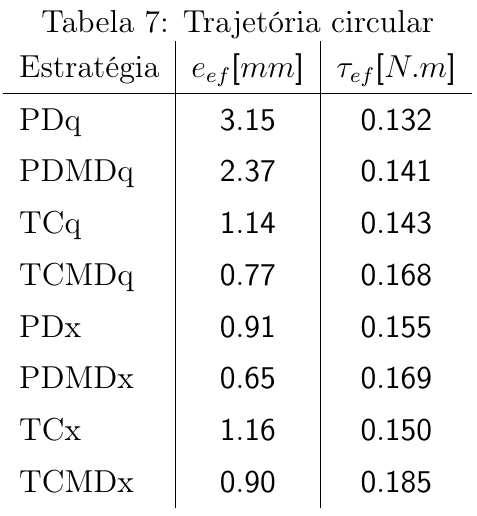
\includegraphics[scale=0.40]{Tabela7.png}
    \end{figure}
\end{frame}

\begin{frame}{Discussão}
    %\framesubtitle{Resultados}
    \begin{figure}[!h]
        \centering
        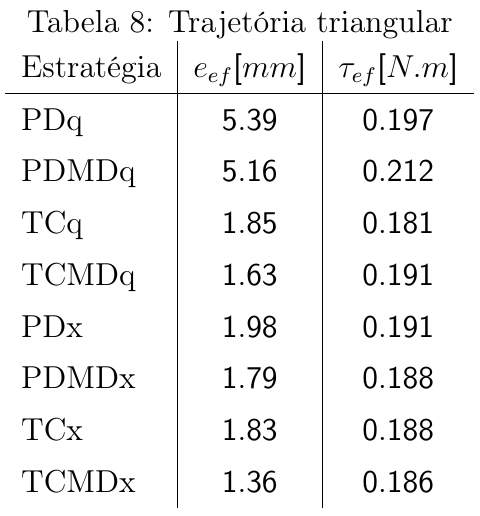
\includegraphics[scale=0.40]{Tabela8.png}
    \end{figure}
\end{frame}

\begin{frame}{Discussão}
    \begin{block}{Combinação com MD}
        \begin{itemize}
            \item[--] Diminuição do $e_{ef}$ em todos os casos \\[5pt]
            \item[--] Diminuição considerável do erro estacionário de posição \\[5pt]
            \item[--] Aumento perceptível do $\tau_{ef}$ na trajetória circular \\[5pt]
            \item[--] Aumento sutil do $\tau_{ef}$ na trajetória triangular \\[5pt]
            \item[--] Diminuição nos valores de pico do erro na trajetória triangular \\[5pt]
            \item[--] Aumento do conteúdo harmônico do esforço de controle \\[5pt]
        \end{itemize}
    \end{block}
    \pause
    \begin{block}{Espaço das juntas vs Espaço da tarefa}
        \begin{itemize}
            \item[--] Desempenho superior do PD e PDMD no espaço da tarefa \\[5pt]
            \item[--] Desempenho equivalente do TC e TCMD em ambos espaços \\[5pt]
        \end{itemize}
    \end{block}
\end{frame}

\begin{frame}{Discussão}
    \begin{block}{Trajetória circular: partida e parada}
        \begin{itemize}
            \item[--] PDx e PDMDx apresentam os menores picos de erro \\[5pt]
            \item[--] Combinação com MD aumenta os valores de pico do erro \\[5pt]
        \end{itemize}
    \end{block}
    \pause
    \begin{block}{Trajetória triangular}
        \begin{itemize}
            \item[--] Para as leis beseadas em modelos, o erro é maior no trecho I \\[5pt]
            \item[--] PDq e PDMDq apresentam maior erro nos trechos I e III \\[5pt]
            \item[--] PDx e PDMDx apresentam maior erro nos trecho II \\[5pt]
            \item[--] Combinação com MD diminui os valores de pico do erro (efeito \emph{undershoot}) \\[5pt]
        \end{itemize}
    \end{block}
\end{frame}

\begin{frame}{Discussão}
    \begin{block}{Consumo energético}
        \begin{itemize}
            \item[--] Valores de $\tau_{ef}$ muito próximos na trajetória triangular \\[4pt]
            \item[--] PDq, PDMDq e TCq apresentam os menores valores de $\tau_{ef}$ na trajetória circular \\[4pt]
            \item[--] TCMDq, PDMDx e TCMDx apresentam os maiores valores de $\tau_{ef}$ na trajetória circular \\[4pt]
        \end{itemize}
    \end{block}
    \pause
    \begin{block}{Erro de controle}
        \begin{itemize}
            \item[--] PDq e PDMDq apresentam os maiores valores de $e_{ef}$ em ambas as trajetórias \\[4pt]
            \item[--] TCMDx e PDMDx apresentam os menores valores de $e_{ef}$ na trajetória circular \\[4pt]
            \item[--] TCMDx e TCMDq apresentam os menores valores de $e_{ef}$ na trajetória triangular \\[4pt]
        \end{itemize}
    \end{block}
\end{frame}

\begin{frame}{Conclusões}
    \begin{block}{}
    	\pause
        \begin{itemize}
            \item[$\bullet$] Algoritmo de modelagem proposto: se mostrou bastante adequado ao seu propósito, facilitando muito o processso de modelagem e implementação do modelo para controle \\[8pt]
            \pause
            \item[$\bullet$] Leis de controle propostas (PDMD e TCMD): também se mostraram bastante adequadas para o controle de mecanismo paralelo, aumentanto o desempenho em relação às leis de controle puras (PD e TC) ao custo de um pequeno aumento no custo computacional e no custo energético \\[8pt]
            \pause
            \item[$\bullet$] A escolha entre espaço das juntas e espaço da tarefa: pode ter grande influência no desempenho do sistema, dependendo da lei de controle escolhida \\[8pt]
        \end{itemize}
    \end{block}
\end{frame}

\begin{frame}{Principais contribuições}
    \begin{block}{}
    	\pause
        \begin{itemize}
            \item[$\bullet$] Desenvolvimento do algoritmo genérico para modelagem dinâmica de manipuladores paralelos translacionais \\[8pt]
            \pause
            \item[$\bullet$] Síntese de uma nova lei de controle não linear robusto para manipuladores robóticos, com desempenho comprovado experimentalmente \\[8pt]
            \pause
            \item[$\bullet$] Avaliação e comparação de desempenho entre 8 diferentes estratégias de controle para manipuladores paralelos através de ensaios experimentais \\[8pt]
        \end{itemize}
    \end{block}
\end{frame}

\begin{frame}{Trabalhos futuros}
    \begin{block}{}
        \begin{itemize}
            \item[$\bullet$] Extensão do algoritmo de modelagem para mecanismos paralelos de até 6 gl no efetuador \\[8pt]
            \pause
            \item[$\bullet$] Obtensão de resultados experimentais das leis de controle propostas em um mecanismo paralelo de atuação redundante (Super-Clara) \\[8pt]
        \end{itemize}
    \end{block}
\end{frame}

\begin{frame}{Agradecimentos}

\end{frame}












%-----------------------------------------------------------------------------------------------------------------------------------

\end{document}